\chapter{ചരിത്രപഠനം കൊണ്ട് എന്തു കാര്യം?}
\label{chapter1}

\begin{center}
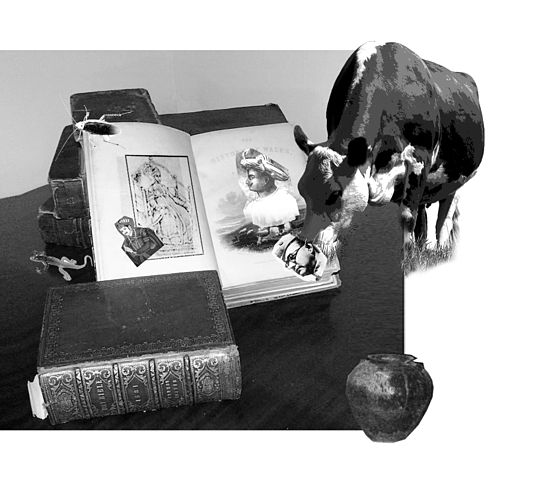
\includegraphics[width=\textwidth,height=10cm]{Kulasthree_Chapter01_pic01.jpg}
\end{center}

\textit{
\paragraph{}
 ഒരു വിഷയമെന്ന നിലയ്ക്ക്, ഒരു തരം വിജ്ഞാനമെന്ന നിലയ്ക്ക്, ചരിത്രം നാമെന്തിനു പഠിക്കണം? ഈ ചോദ്യത്തിന് ഉത്തരം കാണാതെ സ്ത്രീകളുടെ ചരിത്രത്തെക്കുറിച്ച് അന്വേഷിക്കുന്നതിൽ അർത്ഥമില്ല. ചരിത്രമെന്ന പഠനവിഷയത്തെക്കുറിച്ച് നമ്മുടെയിടയിൽ സാധാരണയായി കണ്ടുവരുന്ന തെറ്റിദ്ധാരണകൾ നീക്കാനാണ് ഈ ആമുഖാദ്ധ്യായം ശ്രമിക്കുന്നത്. ഇന്നു പ്രചാരം നേടിയിരിക്കുന്ന പുതിയ ചരിത്രരചനാരീതികളുടെ ഒരു ഏകദേശചിത്രവും ഇവിടെ വരച്ചിടാൻ ശ്രമിക്കുന്നു.}
\section{മാറുന്ന ചരിത്രപഠനം}

\paragraph{}		മലയാളിസ്ത്രീക്ക് അവളുടേതായ ചരിത്രമുണ്ടോ എന്ന് പലരും ചോദിച്ചുതുടങ്ങിയ കാലമാണ് നമ്മുടേത്. നാം ഇന്നത്തെ അവസ്ഥയിൽ എങ്ങനെയെത്തി, പുരോഗമനകേരളത്തിൽ സ്ത്രീകൾ ഇത്രയധികം അവശതകൾ അനുഭവിക്കുന്നതെന്തുകൊണ്ട് മുതലായ ചോദ്യങ്ങൾ കഴിഞ്ഞ കാലങ്ങളിലേക്ക് ഒന്നുകൂടി ഇറങ്ങിച്ചെല്ലാനും പുതിയ ഉത്തരങ്ങൾ തേടാനും നമ്മെ പ്രേരിപ്പിക്കുന്നവയാണ്. ഇത്തരം അന്വേഷണങ്ങൾ കേരളത്തിൽ ഇന്നു പുതുമയല്ല. പക്ഷേ, അവയുടെ ഉൾക്കാഴ്ചകൾ കഴിയുന്നത്ര വായനക്കാരിലേക്ക് എത്തിക്കേണ്ടതാണ്. നമുക്കിന്ന് ലഭ്യമായ സ്ത്രീചരിത്രരചനകളുടെ ഉൾക്കാഴ്ചകളെ കഴിവതും ചുരുക്കി, ലളിതമായഭാഷയിൽ, വായനക്കാരികൾക്ക് എത്തിച്ചു കൊടുക്കുകയെന്നതാണ് ഈ പുസ്തകത്തിന്റെ ലക്ഷ്യം. കൂടാതെ സ്ത്രീചരിത്രപഠനം ആരംഭിക്കാൻ ഉദ്ദേശിക്കുന്ന വിദ്യാർത്ഥികൾക്കും മറ്റുള്ളവർക്കും ഈ പുസ്തകം ഗുണകരമാകണമെന്നും ഉദ്ദേശിക്കുന്നുണ്ട്.

\paragraph{}	ചരിത്രമെന്നാൽ അറുമുഷിപ്പൻ വിഷയമാണെന്ന അഭിപ്രായം നമ്മുടെയിടയിൽ പരക്കെയുണ്ട്. കാണാപ്പാഠം പഠിക്കേണ്ടിവരുന്നതുകൊണ്ട് സ്കൂൾ വിദ്യാർത്ഥികളിൽ വലിയൊരു വിഭാഗത്തിന് ചരിത്രത്തോട് അകൽച്ചയാണ്. പൊതുവേ ബുദ്ധിയില്ലാത്തവർ പഠിക്കുന്ന വിഷയമാണ് ചരിത്രമെന്നുപോലും പല മിടുമിടുക്കികളും മിടുക്കന്മാരും പറഞ്ഞുകേട്ടിട്ടുണ്ട്. ചരിത്രത്തിന് ഇത്രയും ചീത്തപ്പേര് എങ്ങനെ കിട്ടി?
ഇതിന് പല കാരണങ്ങളുണ്ട്. ഒന്നാമതായി, ചരിത്രമെന്നാൽ എന്താണെന്ന ചോദ്യത്തിന് 'കഴിഞ്ഞുപോയകാലത്തിന്റെ കലർപ്പില്ലാത്ത ചിത്രം' എന്ന ഉത്തരമാണ് നമുക്ക് സാധാരണ കിട്ടാറുള്ളത്. അപ്പോൾ സ്വഭാവികമായും നമ്മുടെ സാമാന്യബുദ്ധിയിൽ ഒരു ചോദ്യമുദിക്കുന്നു. കഴിഞ്ഞുപോയതിനെപ്പറ്റി പഠിച്ചിട്ട് എന്തുകാര്യം? രണ്ടാമതായി, ചരിത്രത്തിൽ നാം പഠിക്കുന്നത് എന്തിനെപ്പറ്റിയാണ്? രാജാക്കന്മാർ, മഹാന്മാർ എന്നിവരെപ്പറ്റി. (റാണിമാരും മഹതികളും അധികമൊന്നും പ്രത്യക്ഷപ്പെടാറില്ല). യുദ്ധങ്ങൾ, പടയോട്ടങ്ങൾ, വിപ്ലവങ്ങൾ മുതലായ മഹാസംഭവങ്ങളെപ്പറ്റി. ഇതുകൂടാതെ സമൂഹത്തിലെ ഏറ്റവും ഉയർന്ന തട്ടിലുള്ളവർക്ക് ആസ്വദിക്കാവുന്ന കല, സാഹിത്യം, സംസ്കാരം തുടങ്ങിയവയെപ്പറ്റി. സാധാരണക്കാരുടെ സാധാരണ ജീവിതത്തിന് ചരിത്രമില്ലേയെന്ന് നമ്മൾ ചോദിച്ചുപോകും. അതോ കൃഷിക്കും വീട്ടുജോലിക്കും കൈവേലകൾക്കും ഫാക്ടറിപ്പണികൾക്കും കുട്ടികളെ പ്രസവിക്കലിനും വളർത്തലിനുമൊന്നും ചരിത്രമേയില്ല എന്നാണോ? ഈ ചോദ്യത്തിന് കാര്യമായ ഉത്തരമൊന്നും ക്ലാസ്മുറികളിൽനിന്ന് കിട്ടാറില്ല. പലപ്പോഴും പാഠപുസ്തകങ്ങൾ മെച്ചമാണെങ്കിലും പഠിപ്പിക്കുന്ന രീതി ലവലേശം മാറിയിട്ടില്ല. ഫലമോ, ഇന്നും സ്കൂളുകളിൽ (കലാലയങ്ങളിലും) ചരിത്രപഠനം കാണാപ്പാഠംപഠിത്തവും "തീയതിവിഴുങ്ങലും' മാത്രമായി തുടരുന്നു. ഈ പരാതികൾ ഗൗരവത്തോടുകൂടി കാണേണ്ടവയാണ്. നമുക്ക് ഏറ്റവും ആവശ്യമായ ഒരു വിജ്ഞാനശാഖയാണ് ചരിത്രം. അതു നമ്മളിൽനിന്ന് വളരെ അകലെയാണെന്നാണ് ഈ പരാതികൾ സൂചിപ്പിക്കുന്നത്. ഇതിന് 
എങ്ങനെ സമാധാനം കാണാം?

\paragraph{}		ഒന്നാമത്തെ പ്രശ്നം നോക്കാം. ചരിത്രമെന്നാൽ കഴിഞ്ഞകാലത്തിന്റെ കലർപ്പില്ലാത്ത ചിത്രംമാത്രമാണോ? രണ്ടുകാര്യങ്ങൾ തുടക്കത്തിൽത്തന്നെ വ്യക്തമാകുന്നുണ്ട്:
\begin{enumerate}
\item
 കഴിഞ്ഞകാലത്തെ സമ്പൂർണ്ണമായി വീണ്ടെടുക്കാൻ നമുക്കൊരിക്കലും കഴിയില്ല,
\item ചരിത്രം സമീപകാലംവരെയും സമൂഹത്തിലെ മേലാളവിഭാഗങ്ങളുടെ കുത്തകയായിരുന്നു.
\end{enumerate}

%%%%%BOX%%%%%%
\captionof{mybox}{ചരിത്രരചനയ്ക്കും ചരിത്രമോ?}\label{ch1box1} % place the caption
\begin{tcolorbox}[%
  breakable, % make the box breakable
  arc=0mm, 
  left=1pt, right = 1pt, 
  boxrule=0mm,
  colback = {blue!10}, % since shadow-gray was not defined
] 
{\paragraph{}അതേ! Historiography എന്ന ആശയത്തെ 'ചരിത്രശാസ്ത്രം' എന്നു പരിഭാഷപ്പെടുത്തിക്കാണാറുണ്ട്. എന്നാൽ 'ചരിത്രരചനയുടെ ചരിത്രം' എന്നു പറയുന്നതാവും കൂടുതൽ ഉചിതം. മറ്റേതൊരു ജ്ഞാനശാഖയേയുംപോലെ ചരിത്രവിജ്ഞാനവും കാലത്തിന്റെ ഒഴുക്കിൽ രൂപപ്പെട്ടതാണ്. സാമൂഹ്യ-രാഷ്ട്രീയ-സാംസ്കാരിക മണ്ഡലങ്ങളിലുണ്ടാവുന്ന മാറ്റങ്ങൾ ചരിത്രരചനയെക്കുറിച്ചുള്ള ആശയങ്ങളെയും ചരിത്രപഠന രീതികളെയും സ്വാധീനിക്കുന്നു. ഇങ്ങനെ സംഭവിക്കുന്ന മാറ്റങ്ങളെക്കുറിച്ചുള്ള അറിവിനെയാണ് ഹിസ്റ്റോറിയോഗ്രഫി എന്നു വിളിക്കാറുള്ളത്. മിക്ക ചരിത്രപഠന കോഴ്സുകളിലും ഹിസ്റ്റോറിയോഗ്രഫി പ്രാധാന്യത്തോടുകൂടി പഠിപ്പിക്കുന്നുണ്ട് - ആ പേരിലും അല്ലാതെയും.}
\end{tcolorbox}
%%%%%%%%%%%


\paragraph{}	ഏറ്റവും വിശാലമായി ആലോചിച്ചാൽ കഴിഞ്ഞുപോയ - അതായത്, ഇനി ഒരിക്കലും മടങ്ങിവരാത്ത - കാലത്തെക്കുറിച്ച് പൂർണ്ണമായ അറിവ് മനുഷ്യർക്കു കിട്ടില്ലെന്ന സത്യം അംഗീകരിക്കേണ്ടിവരും. കഴിഞ്ഞുപോയ കാലത്തേക്ക് മടങ്ങിപ്പോയി അന്നത്തെ അവസ്ഥകൾ എന്തൊക്കെയായിരുന്നുവെന്ന് നേരിൽക്കണ്ട് മനസ്സിലാക്കാനുള്ള വിദ്യയൊന്നും മനുഷ്യരുടെ പക്കലില്ലല്ലോ. അതുകൊണ്ട് പൊയ്പ്പോയകാലം ബാക്കിവച്ചിട്ടുള്ള അവശിഷ്ടങ്ങൾ തിരഞ്ഞുപിടിച്ച് പഠിക്കുന്നതിലൂടെയാണ് ഗവേഷകർ ചരിത്രവിജ്ഞാനം ഉണ്ടാക്കുന്നത്. പഴയകാലത്തെ താളിയോലഗ്രന്ഥങ്ങൾ, ശിലാലിഖിതങ്ങൾ, പണ്ടുകാലത്തുള്ളവർ ഉപയോഗിച്ചിരുന്ന വസ്തുക്കൾ മുതലായവയാണ് അവയിൽ ചിലത്. കുറേക്കൂടി സമീപമായ ഭൂതകാലം - അതായത്, ഒരിരുനൂറു-മുന്നൂറു വർഷം മുമ്പു മുതലുള്ള കാലം - പഠിക്കുന്നവർക്ക് കുറേക്കൂടി സൗകര്യമുണ്ട്. കാരണം ഈ കാലത്തെപ്പറ്റി പഠിക്കാനാവശ്യമായ സാമഗ്രികൾ കുറേക്കൂടി ലഭിക്കാൻ സാദ്ധ്യതയുണ്ട്. അപ്പോൾ നമുക്കു തോന്നും കൂടുതൽക്കൂടുതൽ അവശിഷ്ടങ്ങൾ കണ്ടെത്തിയങ്ങനെ വരുമ്പോൾ ഒരുസമയത്ത് പഴയകാലത്തിന്റെ പരിപൂർണ്ണചിത്രം നമുക്ക് കിട്ടുമായിരിക്കും. പക്ഷേ, ഇങ്ങനെ പ്രതീക്ഷിക്കുന്നതിൽ കാര്യമില്ല. കാരണം പഴയകാലത്തിന്റെ - ഭൂതകാലത്തിന്റെ - എന്തെല്ലാം അംശങ്ങളാണ് നഷ്ടപ്പെട്ടുപോയതെന്ന് കൃത്യമായി തിട്ടപ്പെടുത്താൻ നമുക്ക് വഴിയൊന്നുമില്ലല്ലോ.
\begin{figure}[h]
\begin{center}
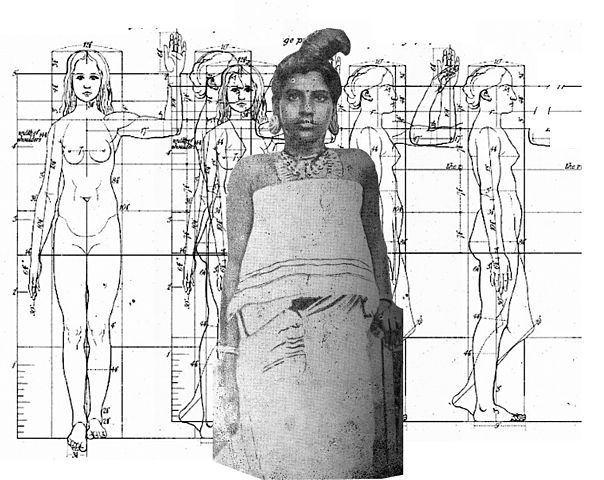
\includegraphics[width=\textwidth,height=10cm]{Kulasthree_Chapter01_pic02.jpg}
\end{center}
\end{figure}



\paragraph{}	'ചരിത്രം' എന്ന വാക്കിന് രണ്ടു പ്രത്യേക അർത്ഥങ്ങളാണ് നാം കല്പിക്കാറ്.
\noindent
\textbf{ഒന്ന്}, കഴിഞ്ഞുപോയകാലം അഥവാ ഭൂതകാലം.
\noindent
\textbf{രണ്ട്}, ആ കഴിഞ്ഞ കാലത്തെക്കുറിച്ച് പഠനത്തിലൂടെ, ഗവേഷണത്തിലൂടെ നാം ഉണ്ടാക്കിയെടുക്കുന്ന അറിവ്. 

	ഈ ഒന്നാമത്തെ അർത്ഥത്തിലുള്ള ചരിത്രത്തെ - ഭൂതകാലത്തെ - രണ്ടാമത്തെ അർത്ഥത്തിലുള്ള ചരിത്രത്തിലൂടെയല്ലാതെ തിരിച്ചറിയാനാവില്ലെന്നതാണ് വാസ്തവം. ചരിത്രഗവേഷണത്തിൽ അവശ്യം പാലിക്കപ്പെടേണ്ട നിബന്ധനകൾക്ക് (ഇവയ്ക്ക് പൊതുവിൽ പറയുന്ന പേരാണ് 'രീതിശാസ്ത്രം') വിധേയമായി ഭൂതകാലത്തെക്കുറിച്ച് നാം തയ്യാറാക്കുന്ന വിജ്ഞാനത്തിനു മാത്രമേ 'ചരിത്രവിജ്ഞാനം' എന്ന അംഗീകാരം കൈവരൂ. എന്നാൽ ചരിത്രപഠനവസ്തുക്കൾ എല്ലായ്പ്പോഴും അപൂർണ്ണങ്ങളായിരിക്കുമെന്നതുകൊണ്ട് ഈ വിജ്ഞാനവും ഭാഗികമായിരിക്കും. മാത്രമല്ല, ചരിത്രം രചിക്കാനുള്ള നിബന്ധനകളിലും പല മാറ്റങ്ങളും സംഭവിച്ചുകൊണ്ടിരിക്കും. അതുകൊണ്ട്, "ഇതാണ് നമ്മുടെ ചരിത്രപാരമ്പര്യം" എന്ന് ആരെങ്കിലും ഉറപ്പിച്ചു പ്രസ്താവിക്കുന്നതു കേട്ടാൽ നാം ഉടനെ ചോദിക്കണം: "ഇന്നത്തെ നിലയ്ക്കുള്ള ചരിത്രഗവേഷണങ്ങളുടെ നിബന്ധനകൾക്കനുസരിച്ച് ഉണ്ടാക്കിയെടുത്തിരിക്കുന്ന അറിവാണോ ഇത്?; ചരിത്രഗവേഷണത്തിനു സഹായകമായ തെളിവുകളുടെ അടിസ്ഥാനത്തിൽ സ്ഥാപിക്കപ്പെട്ട അറിവാണോ ഇത്?"

\begin{center}
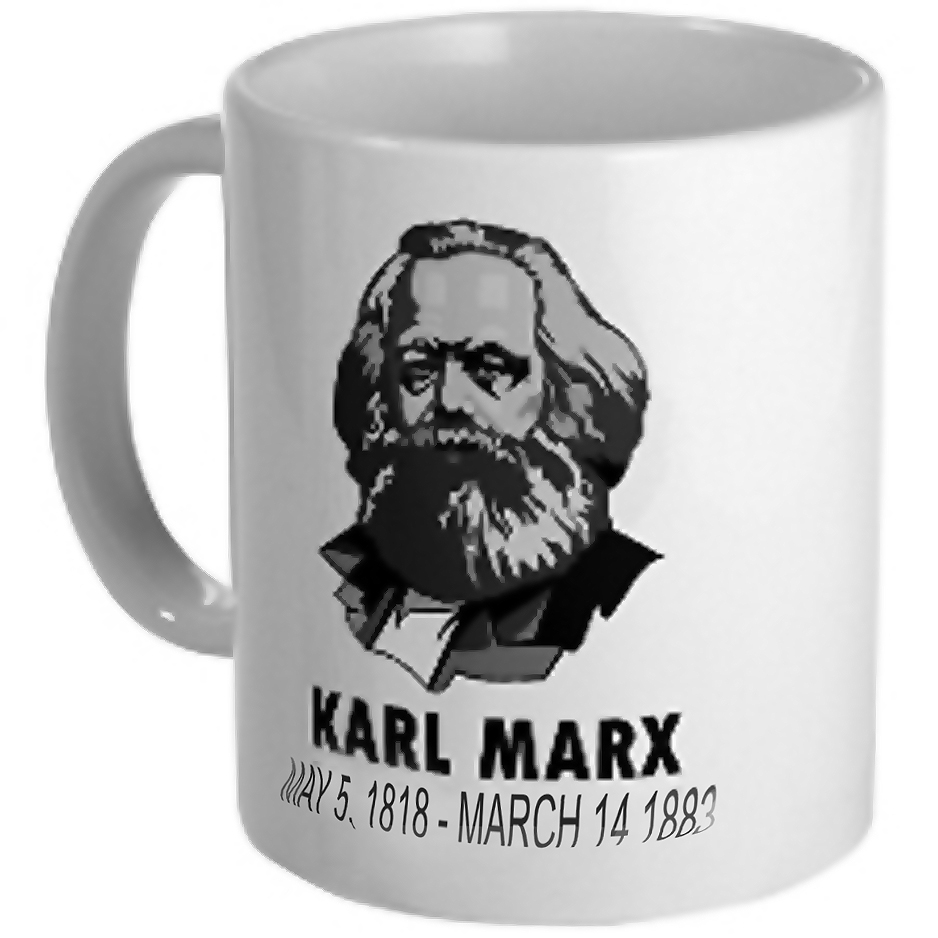
\includegraphics[width=4cm,height=5cm]{Kulasthree_Chapter01_pic03.jpg}
\end{center}

%%%%%BOX%%%%%%
\captionof{mybox}{മാർക്സിസ്റ്റ് ചരിത്രം- മാർക്സിയൻ ചരിത്രം}\label{ch1box2} % place the caption
\begin{tcolorbox}[%
  breakable, % make the box breakable
  arc=0mm, 
  left=1pt, right = 1pt, 
  boxrule=0mm,
  colback = {blue!10}, % since shadow-gray was not defined
] 
{\paragraph{}കാൾ മാർക്സിന്റെ ചിന്തയോട് കടപ്പെട്ടിരിക്കുകയും മാർക്സിസ്റ്റ് രാഷ്ട്രീയപ്രസ്ഥാനങ്ങളെയോ ലക്ഷ്യത്തെയോ പിന്താങ്ങുകയും ചെയ്യുന്ന ചരിത്രപഠനങ്ങളെ Marxist history എന്നു വിളിക്കാറുണ്ടെങ്കിൽ, മാർക്സിസ്റ്റ് ആശയങ്ങളെ ആശ്രയിക്കുന്ന, എന്നാൽ മാർക്സിസ്റ്റ് പ്രസ്ഥാനങ്ങളോടോ രാഷ്ട്രീയത്തോടോ പൂർണ്ണവിധേയത്വമില്ലാത്ത, ചരിത്രരചനയെയാണ് Marxian history എന്ന് വിളിക്കുന്നത്. മനുഷ്യരുടെ ഭൗതികസാഹചര്യങ്ങളിലുണ്ടാകുന്ന മാറ്റങ്ങളനുസരിച്ചാണ് അവരുടെ ചരിത്രത്തിന്റെയും ഗതിമാറുന്നതെന്ന ആശയത്തിന് മാർക്സിസ്റ്റ് ചരിത്രരചനയിൽ സർവ്വപ്രാധാന്യമുണ്ട്. ഒപ്പം, ഭിന്നതാൽപര്യങ്ങളുളള സാമ്പത്തിക-സാമൂഹ്യവർഗ്ഗങ്ങളുടെ ഏറ്റുമുട്ടലുകളാണ് ചരിത്രത്തിന്റെ ഗതിനിർണ്ണയിക്കുന്നതെന്ന് മാർക്സിസ്റ്റ് ചരിത്രരചന അവകാശപ്പെടുന്നു. ഈ രണ്ടു ശക്തികളുടെയും പരിണാമം, പരസ്പരബന്ധം, പ്രതിപ്രവർത്തനം മുതലായവയാണ് മാർക്സിസ്റ്റ് ചരിത്രരചനയുടെ വിഷയങ്ങൾ. നിലവിലുളള അസമവ്യവസ്ഥകളുടെ രൂപീകരണപ്രക്രിയയിലേക്ക് വെളിച്ചംവീശുന്നതുകൊണ്ടുതന്നെ മാർക്സിസ്റ്റ്ചരിത്രം വിമർശനാത്മകവിജ്ഞാനമാകാൻ ശ്രമിക്കുന്ന ജ്ഞാനശാഖയാണ്. ചരിത്രപരമായ ഭൗതികവാദമാണ് (historical materialism) മാർക്സിസ്റ്റ് ചരിത്രവീക്ഷണത്തിന്റെ അന്തഃസത്ത എന്നു പറയാറുണ്ടെങ്കിലും ആ സങ്കല്പത്തെ യാന്ത്രികമായി പ്രയോഗിക്കാൻ സമീപകാല മാർക്സിസ്റ്റ് ചരിത്രരചയിതാക്കൾ അധികവും തയ്യാറല്ല.}
\end{tcolorbox}
%%%%%BOX%%%%%%

\paragraph{}		പഴയകാലത്തിന്റെ അവശിഷ്ടങ്ങളിൽനിന്ന് ഒരുകാര്യം വ്യക്തമാണ് - ഇവ അധികവും പറയുന്നത് അന്നത്തെ സമൂഹത്തിൽ അധികാരവും പണവും പ്രതാപവും ഉണ്ടായിരുന്ന കൂട്ടരെക്കുറിച്ചാണ്. അത് പ്രതീക്ഷിക്കേണ്ടതുതന്നെ. ഇന്നത്തെപ്പോലെ അന്നും ഈടും ഉറപ്പുമുള്ള വസ്തുക്കൾ, വിലപിടിപ്പുള്ള ലോഹങ്ങൾ, എഴുത്തും വായനയും - ഇതെല്ലാം അധികാരിവർഗ്ഗങ്ങളുടെ കൈവശമായിരുന്നുവെന്നത് നേരാണ്. ഇതിനിടയിൽക്കൂടെ അന്നത്തെ പാവപ്പെട്ടവരുടെയും സാധാരണക്കാരുടെയും ജീവിതത്തെക്കുറിച്ച് വളരെക്കുറച്ചു വിവരമേ നമുക്ക് കിട്ടുന്നുള്ളു. അതുതന്നെ അധികാരിവർഗ്ഗങ്ങളുടെ കണ്ണിലൂടെയാണ് നമ്മളിലേക്ക് എത്തുന്നത്. ഇങ്ങനെ മേലാളരുടെ ഭൂതകാലത്തിലേക്ക് വെളിച്ചംവീശുന്ന ചരിത്രസാമഗ്രികൾക്കപ്പുറം സാധാരണജനങ്ങളുടെ ജീവിതത്തിന്റെ ചരിത്രം പഠിക്കാനുതകുന്ന സാമഗ്രികളെക്കുറിച്ച് ആരായേണ്ടതാണെന്ന ബോധംപോലും താരതമ്യേന സമീപകാലത്തുമാത്രമുണ്ടായതാണ്. പുരാതനസമുദായങ്ങളുടെ ഉത്ഖനനങ്ങളിൽനിന്ന് വൈവിദ്ധ്യമാർന്ന വസ്തുക്കൾ കണ്ടെത്തിയിട്ടുണ്ട്. എന്നാൽ സംസ്കൃതികളുടെ സവിശേഷതകളെക്കുറിച്ചറിയാനുള്ള ആവേശത്തിനുപരിയായി സാധാരണജനങ്ങളുടെ ജീവിതത്തെക്കുറിച്ചുള്ള ജിജ്ഞാസ ചരിത്രരചനാരംഗത്ത് സാർവ്വത്രികമായത് താരതമ്യേന സമീപകാലത്താണ്. അടുത്തകാലംവരെയും മേലാളവർഗ്ഗക്കാരുടെ ചരിത്രത്തെയാണ് ഇന്ത്യാചരിത്രം, കേരളചരിത്രം, ലോകചരിത്രം എന്നൊക്കെയുള്ള വിശാലമായ തലക്കെട്ടുകളിലൂടെ അവതരിപ്പിച്ചുകൊണ്ടിരുന്നത്. ഈ ചരിത്രത്തെ 'നിഷ്പക്ഷചരിത്രം' എന്ന ലേബലോടുകൂടിയാണ് മിക്ക പാഠപുസ്തകങ്ങളും അവതരിപ്പിക്കുന്നത്.

\paragraph{}	ലോകത്തെമ്പാടും അധികാരമില്ലാത്ത ജനങ്ങൾക്കുവേണ്ടി സമരംചെയ്ത ഇടതുപക്ഷപ്രസ്ഥാനങ്ങൾ വളർന്നതിനൊപ്പം, പണിയെടുക്കുന്ന വർഗ്ഗങ്ങളുടെ ചരിത്രവും രൂപപ്പെട്ടുതുടങ്ങിയെന്നത് നേരുതന്നെ. മാർക്സിസ്റ്റ് ചരിത്രരചനയിൽ കർഷകർ, തൊഴിലാളികൾ, അടിമകൾ, മേലാളർക്കെതിരെ സമരംചെയ്ത അടിയാളർ മുതലായവരുടെ ചരിത്രാനുഭവങ്ങളെക്കുറിച്ചുള്ള അന്വേഷണം സജീവമായി. മാർക്സിസ്റ്റ് ചരിത്രരചനയിൽ മഹാന്മാരുടെ ചെയ്തികൾക്കപ്പുറം മുതലാളിത്തവ്യവസ്ഥയുടെ രൂപീകരണത്തിന്റെ ഫലമായി ശക്തിപ്രാപിച്ച അധികാരരൂപങ്ങൾ, ആശയസമുച്ചയങ്ങൾ, സാമ്പത്തികപ്രയോഗങ്ങൾ, രാഷ്ട്രീയ സംഘർഷങ്ങൾ, പുതിയ സ്ഥാപനങ്ങൾ എന്നിവയെക്കുറിച്ചുള്ള ഗവേഷണത്തിന് പ്രാധാന്യം കൈവന്നു. എങ്കിലും പണിയെടുക്കുന്നവരുടെ ചരിത്രങ്ങൾ എഴുതിയവർ എല്ലാ തൊഴിലാളികൾക്കും ഒരേ പ്രാധാന്യം കൊടുത്തില്ല. സമൂഹത്തെ മുന്നോട്ടുനയിക്കുന്നത് തൊഴിലാളികളാണെന്ന ബോധമായിരുന്നു ഇടതുപക്ഷചരിത്രരചനയ്ക്ക് പലപ്പോഴും പ്രചോദനമായത്. എന്നാൽ ഇവിടെയും സംഘടനകളിലൂടെ ശക്തരായിത്തീർന്ന തൊഴിലാളികൾക്കാണ് പ്രാധാന്യംകിട്ടിയത്. തൊഴിലാളികളിൽ വലിയൊരു വിഭാഗം സ്ത്രീകളായിരുന്നിട്ടും അവർ അപ്പോഴും അദൃശ്യരായിത്തന്നെയിരുന്നു. എന്നാൽ ഇന്ന് മേലാള-മാർക്സിസ്റ്റ് ചരിത്രത്തിന്റെ പരിമിതികളെ മറികടക്കാൻ ശ്രമിക്കുന്ന ചരിത്രരചനാധാരകൾ അനവധിയാണ്.

\paragraph{}	പാഠപുസ്തകങ്ങളിൽ നാം പഠിക്കുന്ന 'നിഷ്പക്ഷചരിത്ര'ത്തിന് താഴെപ്പറയുന്ന അഞ്ചു പ്രധാന ധാരണകളാണുള്ളത്. അഞ്ചും കാലഹരണപ്പെട്ടുകഴിഞ്ഞുവെന്ന് പുതുചരിത്രകാരന്മാരും ചരിത്രകാരികളും പറയുന്നുണ്ടെങ്കിലും, പലയിടങ്ങളിലും പഠനസമ്പ്രദായത്തിൽ മാറ്റംവരുത്താൻ ശ്രമം നടക്കുന്നെങ്കിലും, ഇന്നും ചരിത്രത്തെക്കുറിച്ചുളള സാമാന്യബോധം ഇതൊക്കെത്തന്നെയാണ്.

\begin{figure}
\begin{center}
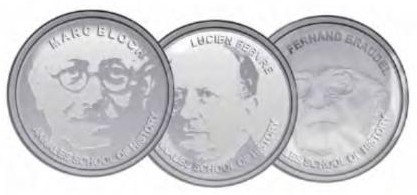
\includegraphics[width=8cm,height=4cm]{Kulasthree_Chapter01_pic04.jpg}
\end{center}
\end{figure}


\begin{enumerate}
\item
		ഭൂതകാലംമുതൽ വർത്തമാനകാലംവരെ നടന്നിട്ടുളള ചരിത്രസംഭവങ്ങളെ അവയുടെ കാലമനുസരിച്ച് ക്രമത്തിൽ അടുക്കിപ്പറയുന്ന രീതിയാണ് ഉത്തമ ചരിത്രരചനയുടെ ലക്ഷണം. മറ്റൊരുവിധത്തിൽപ്പറഞ്ഞാൽ, ചരിത്രരചനയെന്നാൽ ചരിത്രസംഭവങ്ങളെ സംഭവിച്ച ക്രമമനുസരിച്ച് കോർത്തിണക്കി അവതരിപ്പിക്കുന്ന പറച്ചിൽ അഥവാ ആഖ്യാനമാണ്.
 \item
ചരിത്രരചന ഏറ്റവുമധികം പ്രാധാന്യം നൽകേണ്ടത് ദേശീയരാഷ്ട്രീയരംഗത്തുണ്ടാകുന്ന മാറ്റങ്ങൾക്കാണ്
\item
ചരിത്രമെപ്പോഴും മുകളിൽനിന്നുള്ള ചരിത്രമാണ്. അതായത് ഭരണാധികാരിവർഗ്ഗത്തിന്റെ വീക്ഷണത്തിൽനിന്നും എഴുതപ്പെടുന്ന, ഭരണാധികാരിവർഗ്ഗത്തിന്റെ വികസനപരിണാമങ്ങൾക്ക് ഊന്നൽ നൽകുന്ന ആഖ്യാനമാണ് ചരിത്രം.
\item ഔദ്യോഗികരേഖകളെയും ആധികാരിക പുരാവസ്തു-പുരാരേഖാശേഖരങ്ങളെയും ആശ്രയിക്കുന്ന ചരിത്രരചനയാണ് ഉത്തമസ്വഭാവമുളളത്. ഔദ്യോഗികരേഖകൾ ഭരണാധികാരത്തിന്റെ കണ്ണിലൂടെ സൃഷ്ടിക്കപ്പെടുന്നവയാണെന്ന് പ്രത്യേകിച്ച് പറയേണ്ടതില്ലല്ലോ.
\item ചരിത്രപുരുഷന്മാരുടെ പ്രവൃത്തികൾ മനസ്സിലാക്കാൻ അവരുടെ മനോവ്യാപാരങ്ങൾ, വിശ്വാസങ്ങൾ, അവർ സ്വീകരിച്ചിരുന്ന ആശയങ്ങൾ ഇതൊക്കെ മനസ്സിലാക്കിയാൽ മതി. അല്ലാതെ അവർ ജീവിച്ചിരുന്ന വിശാലപശ്ചാത്തലത്തിന്റെ പ്രസക്തിയോ മറ്റു സങ്കീർണ്ണതകളോ കണക്കാക്കേണ്ടതില്ല.
\end{enumerate}

\paragraph{}	മേൽപ്പറഞ്ഞ അഞ്ചു തത്ത്വങ്ങളും അടിമുടി ചോദ്യംചെയ്യപ്പെടുന്ന കാലത്താണ് നാം ജീവിക്കുന്നത്. മാർക്സിസ്റ്റ്ചിന്തയെ ആധാരമാക്കി ചരിത്രരചന നടത്തിയവർ വളരെ മുമ്പുതന്നെ ഇവയെ തള്ളിക്കളഞ്ഞിരുന്നു. എങ്കിലും തൊഴിലാളിവർഗ്ഗത്തിന്റെ ഭാഗമായി അംഗീകരിക്കപ്പെടാത്തവർക്ക് അപ്പോഴും ചരിത്രത്തിനു പുറത്തുതന്നെ നിൽക്കേണ്ടിവന്നു. തൊഴിലാളിവർഗ്ഗത്തിന്റെ ചരിത്രമെന്നതിനപ്പുറം അധികാരമില്ലാത്തവരുടെ ചരിത്രത്തിന് വേറേതന്നെ പ്രാധാന്യമുണ്ടെന്ന് ചരിത്രഗവേഷകർക്കും വിദ്യാർത്ഥികൾക്കും ബോദ്ധ്യംവന്നത് പിന്നീടാണ്. കീഴാളജനങ്ങളുടെ (അധികാരം നിഷേധിക്കപ്പെട്ട ജനവിഭാഗങ്ങളാണ് കീഴാളർ - സ്ത്രീകൾ, അടിമകൾ, കീഴ്ജാതിക്കാർ, പാവപ്പെട്ടവർ, തൊഴിലാളികൾ) ചരിത്രങ്ങൾ പഠിക്കാൻ പുതിയ ശ്രമങ്ങൾ ഇന്നുണ്ട്. കൂടുതൽ സൂക്ഷ്മമായ വായനയിലൂടെയും പുതിയ ചരിത്രസാമഗ്രികൾ കണ്ടെത്തുന്നതിലൂടെയും കീഴാളചരിത്രാന്വേഷികൾ ചരിത്രപഠനത്തിന്റെ മുഖംതന്നെ മാറ്റിയെഴുതുകയാണ്. എന്നാൽ ഇത്തരം ശ്രമങ്ങൾക്ക് ആക്കംകൂടിയത് അടുത്തകാലത്താണ്.

%%%%%BOX%%%%%%
\captionof{mybox}{നിഷ്പക്ഷചരിത്ര'ത്തിന്റെ മറ്റു വിമർശകർ}\label{ch1box3} % place the caption
\begin{tcolorbox}[%
  breakable, % make the box breakable
  arc=0mm, 
  left=1pt, right = 1pt, 
  boxrule=0mm,
  colback = {blue!10}, % since shadow-gray was not defined
] 
{\paragraph{}മാർക്സിസ്റ്റുകൾക്കു പുറമേ 'നിഷ്പക്ഷചരിത്ര'ത്തിന്റെ പരിമിതികളെക്കുറിച്ച് ശക്തമായ വിമർശനമുന്നയിച്ച പ്രമുഖരായിരുന്നു Marc Bloch, Lucien Febvre, Fernand Braudel എന്നീ ഫ്രഞ്ച് ചരിത്രകാരന്മാർ. ഇവർ വളർത്തിയെടുത്ത ചരിത്രരചനാസമ്പ്രദായത്തെ Annales School of History എന്ന് വിളിക്കുന്നു. രാഷ്ട്രീയ സംഭവങ്ങൾക്കു നൽകുന്ന അമിതപ്രാധാന്യത്തെ എതിർത്ത ഇവർ സാമ്പത്തിക-സാംസ്കാരികചരിത്രത്തിന് മുന്തിയ സ്ഥാനംനൽകി. പള്ളി ഇടവക രേഖകൾ, ചന്തകളും മറ്റു വ്യാപാരകേന്ദ്രങ്ങളുമായി ബന്ധപ്പെട്ട രേഖകൾ മുതലായവ കഴിഞ്ഞകാലത്തെക്കുറിച്ച് വിലപ്പെട്ട അറിവ് നൽകുന്നവയാണെന്ന് സ്ഥാപിച്ചു. സാധാരണജനങ്ങളുടെ ദൈനംദിനജീവിതത്തിന്റെ പ്രാധാന്യത്തിന് ഊന്നൽകൊടുത്തു. രാഷ്ട്രീയചരിത്രമല്ല സാമൂഹ്യജീവിതത്തിന്റെ എല്ലാ വശങ്ങളെക്കുറിച്ചും പഠിക്കുന്ന 'സമ്പൂർണ്ണചരിത്രം' (total history) ആയിരിക്കണം ചരിത്രരചനയുടെ ലക്ഷ്യമെന്ന് Braudel അഭിപ്രായപ്പെട്ടു. മൂന്നുതരം കാലഗണനാതലങ്ങൾ സ്വീകരിച്ചുകൊണ്ടായിരിക്കണം ഇതെന്ന് അദ്ദേഹം അഭിപ്രായപ്പെട്ടു: ഒന്ന്, 'ഘടന/പാരമ്പര്യം' (structure) എന്ന തലം. ഇത് ഏറ്റവും അടിസ്ഥാനപരവും ഏറ്റവും സാവധാനംമാത്രം മാറുന്നതുമായ തലമാണ് - നൂറ്റാണ്ടുകളോളം നില നിൽക്കുന്നത്. രണ്ട്, 'പ്രവണത' അഥവാ conjuncture. ഇത് ഒന്നുരണ്ടു തലമുറ നീളുന്ന കാലയളവാണ്. മൂന്ന്, 'സംഭവം' അഥവാ event. അതിവേഗം മാറുന്ന തലമാണിത്; നേരിട്ട് കണ്ടെത്താനാവുന്നതും. ആദ്യതലം 'കടലിലെ അടിയൊഴുക്കുകൾ' പോലെയും, രണ്ടാമത്തെ തലം 'കടലിലെ വേലിയേറ്റ-വേലിയിറക്കങ്ങൾ' പോലെയും മൂന്നാമത്തെ തലം 'കടലിലെ തിരമാലകൾ' പോലെയും ആണെന്നാണ് അദ്ദേഹത്തിന്റെ അഭിപ്രായം.}
\end{tcolorbox}

%%%%%BOX%%%%%%



\paragraph{}	ഇന്ന് വളർന്നുകൊണ്ടിരിക്കുന്ന ഈ പുതിയ ചരിത്രവിജ്ഞാനം നമ്മുടെയിടയിൽ വേണ്ടത്ര എത്തിയിട്ടില്ല. ഇപ്പോഴും നമ്മുടെ സ്കൂളുകളിലെ ചരിത്രപഠനത്തിന്റെ ലക്ഷ്യം ഭൂതകാലത്തിന്റെ കലർപ്പില്ലാത്ത, അല്ലെങ്കിൽ നിഷ്പക്ഷമായ ചരിത്രംപഠിക്കൽ തന്നെയാണ്. അപ്പോൾ ചരിത്രമെന്നാൽ മഹാന്മാരും രാജാക്കന്മാരും അവരുടെ ചെയ്തികളുമാണെന്ന് നമ്മൾ ധരിക്കാനിടവന്നത് ചുമ്മാതല്ല. മഹാന്മാരിൽ പലരും ജനസമ്മതിയുള്ളവരായിരുന്നുവെന്നതിൽ തർക്കമില്ല. (ഗാന്ധിജി, പണ്ഡിറ്റ് നെഹ്രു മുതലായവർ ഉദാഹരണം) എന്നാൽ, ഇവരോട് ഒപ്പത്തിനൊപ്പം പ്രധാനികളായി നിന്നിരുന്ന കീഴ്ജാതിനേതാക്കൾക്കോ സ്ത്രീകൾക്കോ പല പുസ്തകങ്ങളിലും വേണ്ടത്ര പ്രാധാന്യം കിട്ടാതെപോകുന്നത് എന്തുകൊണ്ടാണെന്ന് നാം ആലോചിക്കണം. കീഴാളരുടെ ഭൂതകാലത്തെക്കുറിച്ച് അറിവുനൽകുന്ന ചരിത്രവസ്തുക്കൾ കുറവാണെന്നു സമ്മതിക്കാം. എങ്കിലും ഈ കുറവിനെ വലിയൊരളവുവരെ പരിഹരിച്ച് മുന്നോട്ടുപോകാനാകുമെന്ന് അടുത്തകാലങ്ങളിൽ ഗവേഷകർ നിർമ്മിച്ച കീഴാളചരിത്രങ്ങൾ തെളിയിക്കുന്നു. ഇന്ന് പ്രചാരത്തിലിരിക്കുന്ന ഔദ്യോഗികചരിത്രം (അത് ഇന്ത്യയുടേതായാലും ശരി, കേരളത്തിന്റേതായാലും ശരി) അവകാശപ്പെടുന്ന നിഷ്പക്ഷത മേലാളചരിത്രത്തിനുള്ള മറ മാത്രമാണെന്ന് ചരിത്രഗവേഷകർ ചൂണ്ടിക്കാട്ടുന്നു.

	\paragraph{}	പൊതുവേ ഈ മാറ്റങ്ങൾ 'നിഷ്പക്ഷചരിത്ര'ത്തിന്റെ വക്താക്കളെ വളരെ ചൊടിപ്പിക്കുന്നുണ്ട്. ചരിത്രമെന്നാൽ പഴയകാലത്തിന്റെ കലർപ്പില്ലാത്ത ചിത്രമല്ലെന്നു പറയുമ്പോൾ അവർ ചോദിക്കാറുണ്ട്, 'ഓ, പിന്നെ അതെന്താ കെട്ടുകഥയാണോ?' തീർച്ചയായും 'അല്ല' എന്നാണ് ഈ ചോദ്യത്തിനു മറുപടി. നേരത്തെ സൂചിപ്പിച്ചതുപോലെ പുതിയ തെളിവുകളുടെ അടിസ്ഥാനത്തിലാണ് ഈ പുതിയ ചരിത്രരചനകൾ ഉണ്ടായിരിക്കുന്നത്. വ്യക്തമായ തെളിവുകളുടെ അടിസ്ഥാനമെന്തായിരിക്കുമെന്ന ചോദ്യം ചരിത്രപണ്ഡിതർ ഇന്നും ചർച്ചചെയ്യുന്ന ഒന്നാണെങ്കിലും, വിശ്വസിക്കാവുന്ന വാദങ്ങൾ എങ്ങനെ നിർമ്മിക്കാമെന്നതിനെപ്പറ്റി ചില പൊതുസമ്മതങ്ങൾ അവർക്കിടയിലുണ്ട്. എന്നാൽ, എന്തൊക്കെ നല്ല തെളിവായി കണക്കാക്കാമെന്നതിനെപ്പറ്റി പഴയരീതിയിൽ ചിന്തിക്കുന്ന ചരിത്രകാരന്മാരും പുതിയ രീതിയിൽ ചിന്തിക്കുന്നവരും തമ്മിൽ അഭിപ്രായവ്യത്യാസമുണ്ടെന്നതു നേരു തന്നെ. ഇക്കാര്യത്തെപ്പറ്റി പൂർണ്ണമായ അഭിപ്രായ ഐക്യം ഇല്ലാത്തതുകൊണ്ടുതന്നെ നിരവധി ചരിത്രരചനാധാരകളും വ്യത്യസ്ത രചനാപദ്ധതികളും നിലവിലുണ്ട്. ഇവ തമ്മിലുള്ള നിരന്തരസംവാദങ്ങളിലൂടെയാണ് ചരിത്രവിജ്ഞാനം വിസ്തൃതമാകുന്നത്. ഇത്തരം സംവാദത്തിലൂടെ, അനവധി ഗവേഷകരുടെ സൂക്ഷ്മപരിശോധനയിലൂടെ കടന്ന ചരിത്രസാമഗ്രികൾക്കുമാത്രമെ തെളിവെന്ന സമ്മതം ലഭിക്കൂ. വേണ്ടത്ര, തക്കതായ തെളിവില്ലാതെ നല്ല ചരിത്ര രചന നടക്കില്ല. ഇടുങ്ങിയ സ്ഥാപിതതാൽപര്യങ്ങളെ താങ്ങിനിർത്താൻവേണ്ടി എഴുതപ്പെടുന്ന ചരിത്രങ്ങളുടെ ചെമ്പ് പെട്ടെന്നുതന്നെ തെളിയുന്നത് ഇതിനാലാണ്.

\begin{figure}[h]
\begin{center}
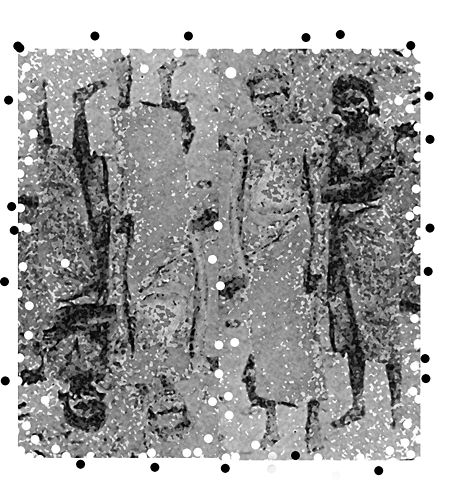
\includegraphics[width=\textwidth,height=10cm]{Kulasthree_Chapter01_pic05.jpg}
\end{center}
\end{figure}



%%%%%BOX%%%%%%
\captionof{mybox}{കീഴാളപഠനങ്ങൾ അഥവാ Subaltern Studies}\label{ch1box4} % place the caption
\begin{tcolorbox}[%
  breakable, % make the box breakable
  arc=0mm, 
  left=1pt, right = 1pt, 
  boxrule=0mm,
  colback = {blue!10}, % since shadow-gray was not defined
] 
{\paragraph{}ബ്രിട്ടിഷ് അധികാരത്തിനെതിരെ ഇന്ത്യയുടെ പല ഭാഗങ്ങളിലേയും കീഴാളവിഭാഗങ്ങൾക്കിടയിൽനിന്നുണ്ടായ എതിർപ്പിനെ സാമ്പ്രദായികചരിത്രരചനാരീതികൾ അധികവും അവഗണിക്കുകയാണുണ്ടായത്. ദേശീയപ്രസ്ഥാനത്തിന് കേന്ദ്രപ്രാധാന്യം കല്പിച്ച ദേശീയവാദചരിത്രമോ (Nationalist history) മാർക്സിസ്റ്റ് ചരിത്രമോ പോലും വേണ്ടത്ര പ്രാധാന്യം ഈ ചെറുത്തുനില്പുകൾക്ക് നൽകിയില്ല. ഈ തമസ്കരണത്തിനെതിരെയുളള നീക്കമാണ് 'കീഴാളപഠനങ്ങൾ' എന്ന് ആ പ്രസ്ഥാനത്തിന്റെ വക്താക്കൾ അവകാശപ്പെടുന്നു. ഔദ്യോഗികരേഖകളിലും ദേശീയ-മാർക്സിസ്റ്റ് ചരിത്രത്തിലും നിശബ്ദരാക്കപ്പെട്ട, അല്ലെങ്കിൽ പാർശ്വവൽക്കരിക്കപ്പെട്ട, ജനവിഭാഗങ്ങളുടെ ചെറുത്തുനിൽപ്പുകളെ വെളിച്ചത്തുകൊണ്ടുവരിക, അവരുടെ അധിനിവേശവിരുദ്ധനിലപാടുകളുടെയും തന്ത്രങ്ങളുടെയും വ്യത്യസ്തത അടയാളപ്പെടുത്തുക മുതലായ ലക്ഷ്യങ്ങളായിരുന്നു ഈ സംഘത്തിന്റേത്. ഔദ്യോഗികരേഖകളെ വരികൾക്കിടയിലൂടെ വായിച്ചും പുതിയ ചരിത്രസ്രോതസ്സുകൾ കണ്ടെത്തിയും മറ്റുമാണ് 'കീഴാളചരിത്രം' മുന്നേറിയത്. 'കീഴാളചരിത്ര'ത്തിന്റെ മറ്റൊരു ധാര, ജാതി/ജന്മിത്തവിരുദ്ധസമരങ്ങളെ ദേശീയസമരത്തിന്റെ ഉപവിഭാഗമായി ചുരുക്കുന്ന വ്യവസ്ഥാപിതരീതിയെ ശക്തമായി എതിർത്തു.}
\end{tcolorbox}
%%%%%BOX%%%%%%

\paragraph{}	അത്തരം അവകാശവാദങ്ങൾ മിക്കപ്പോഴും മതിയായ തെളിവിനെ ആസ്പദമാക്കുന്നവയല്ല. നിലവിൽ അംഗീകരിക്കപ്പെട്ട തെളിവുകളെയും അനുമാനരീതികളെയും അവ കണക്കാക്കുകയുമില്ല. അതുപോലെ, 'പല ചരിത്രകാരന്മാരും പലതും പറയുന്നു, ആരു പറയുന്നത് വിശ്വസിക്കും' എന്ന ചോദ്യവും കേൾക്കാറുണ്ട്. നേരത്തേ പറഞ്ഞതുപോലെ, സമൂഹത്തിലെ മനുഷ്യർക്കു മുഴുവൻ ഒരൊറ്റ ചരിത്രമല്ല ഉള്ളത്. (സാധാരണഗതിയിൽ, ആ പേരിൽ വാഴിക്കപ്പെടുന്നത് മേലാള ചരിത്രമാണെന്ന് പറഞ്ഞല്ലോ) ചരിത്രമെന്നാൽ പല ജനവിഭാഗങ്ങളുടെ പ്രത്യേകമായ ഭൂതകാലങ്ങളെക്കുറിച്ചുള്ള അറിവിന്റെ മേഖലയാണെന്നും ഇന്നു നമുക്കറിയാം. അങ്ങനെയാണെങ്കിൽ ആരു പറയുന്നതു വിശ്വസിക്കുമെന്ന പ്രശ്നം അത്ര ഗുരുതരമാകില്. ഏതെങ്കിലുമൊരു വിഭാഗത്തിന്റെ ചരിത്രത്തിൽ ഭൂതകാലത്തെക്കുറിച്ചുള്ള മുഴുവൻ സത്യവുമുണ്ടെന്ന ധാരണ ശരിയല്ലെന്നു സാരം. ചരിത്രത്തിലെ ശരിയേത്, തെറ്റേത് എന്നും മറ്റുമുള്ള ധാരണകൾ ഓരോ ജനവിഭാഗത്തിലും വ്യത്യസ്തമാവുമെന്നത് സ്വാഭാവികംമാത്രം. രാജാക്കന്മാരുടെ ചരിത്രത്തിലെ ശരിതെറ്റുകൾ പ്രജകളുടെ ചരിത്രത്തിലെ ശരിതെറ്റുകളിൽനിന്നും വിഭിന്നമായിരിക്കും. ഏതെങ്കിലുമൊരു രാജവംശത്തിന്റെ അധികാരമുറപ്പിക്കുന്ന 'മഹത്തായ' യുദ്ധവിജയങ്ങളെ, ആ യുദ്ധത്തിൽ ആളും അർത്ഥവും നഷ്ടപ്പെട്ടു നരകിച്ച ജനങ്ങളുടെ കണ്ണിലൂടെ വിലയിരുത്തിയാൽ തീർത്തും വിഭിന്നമായ കാഴ്ചയാവും നാം കാണുക.
\begin{figure}
\begin{center}
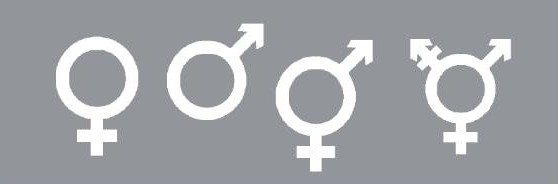
\includegraphics[width=8cm,height=2cm]{Kulasthree_Chapter01_pic06.jpg}
\end{center}
\end{figure}

%%%%%BOX%%%%%%
\captionof{mybox}{ലൈംഗികതയ്ക്കും ആൺ-പെൺഭേദത്തിനും ചരിത്രമോ?}\label{ch1box5} % place the caption
\begin{tcolorbox}[%
  breakable, % make the box breakable
  arc=0mm, 
  left=1pt, right = 1pt, 
  boxrule=0mm,
  colback = {blue!10}, % since shadow-gray was not defined
] 
{\paragraph{}സ്ത്രീത്വം മാത്രമല്ല പുരുഷത്വവും കാലത്തിൽ മാറുന്ന ആശയവും പ്രയോഗവുമാണെന്നും അതിന്റെ ചരിത്രത്തെക്കുറിച്ചും അന്വേഷിക്കേണ്ടതാണെന്നും പലരും വാദിച്ചുതുടങ്ങിയിരിക്കുന്നു. ലൈംഗികാകർഷണവും ആഗ്രഹവും നാം പലപ്പോഴും കരുതുംപോലെ പ്രജനനത്തിനുവേണ്ടി മാത്രമല്ല. അവ പ്രകൃതി നിർണ്ണയിക്കുന്നവയുമല്ല. മറിച്ച് മനുഷ്യരുടെ മാറിവരുന്ന ഭൗതികവും ആശയപരവുമായ സാഹചര്യങ്ങളും ലൈംഗികചോദനകളുടെ രൂപീകരണത്തെ കാര്യമായി നിർണ്ണയിക്കുന്നുണ്ടെന്ന് ഈ ചരിത്രരചയിതാക്കൾ തെളിയിച്ചു. സമൂഹത്തിൽ നിലനിൽക്കുന്ന പലതരം ലൈംഗികചോദനകൾക്കും ആഗ്രഹങ്ങൾക്കും ഒരുപോലെ അംഗീകാരം ലഭിക്കാത്തതെന്തുകൊണ്ട് എന്ന ചോദ്യമാണ് ഇവരുടെ അന്വേഷണങ്ങളെ നയിച്ചത്. 'ലൈംഗികമാന്യത'യ്ക്ക് തീരെ മാന്യമല്ലാത്ത ചരിത്രമാണുള്ളതെന്ന് ഇവരുടെ ചരിത്രരചനകൾ സംശയാതീതമായി തെളിയിക്കുന്നു. സ്വവർഗ്ഗത്തെ സ്നേഹിക്കുന്നവർ, ഹിജഡകൾ, ലിംഗസ്വഭാവമാറ്റത്തിനു വിധേയരാകാനാഗ്രഹിക്കുന്നവർ - ഇങ്ങനെ വ്യവസ്ഥാപിത ലൈംഗികമൂല്യങ്ങളിൽനിന്നു വ്യത്യാസപ്പെട്ടവർ - അനുഭവിച്ച ഹിംസയുടെയും ചൂഷണത്തിന്റെയും ഒപ്പം അവരുടെ ചെറുത്തുനിൽപ്പുകളുടെയും ചരിത്രം ഇന്ന് പുതിയൊരു ലൈംഗികരാഷ്ട്രീയബോധത്തിന് അടിത്തറയിട്ടിരിക്കുന്നു.}
\end{tcolorbox}
%%%%BOX%%%%%%


\paragraph{}	ലോകത്തിന്റെ മറ്റു ഭാഗങ്ങളിലെ ചരിത്രരചനാസമ്പ്രദായങ്ങളിലുണ്ടായ ഗുണകരമായ മാറ്റങ്ങളുടെ അലയൊലികൾ ഇവിടെയും എത്തിയിരിക്കുന്നതിനെപ്പറ്റി പറഞ്ഞല്ലോ. ഇരുപതാം നൂറ്റാണ്ടിന്റെ രണ്ടാംപകുതിയിൽ ലോകമെമ്പാടുമുളള കീഴാളർക്കുണ്ടായ രാഷ്ട്രീയ ഉണർവിന്റെ ഭാഗമായിരുന്നു ഇത്. സ്ത്രീകളെ സംബന്ധിച്ചിടത്തോളം ഈ കാലം നിർണ്ണായകമായിരുന്നു. അതുവരെ മേലാളചരിത്രങ്ങളിലും കർഷക-തൊഴിലാളി ചരിത്രങ്ങളിലും പരിമിതമായ സാന്നിദ്ധ്യംമാത്രമേ അവർക്കുണ്ടായിരുന്നുള്ളൂ. സ്ത്രീകളുടെ ചരിത്രപഠനത്തിനാവശ്യമായ സാമഗ്രികൾ കുറവായിരുന്നു. പൊതുരംഗം, രാഷ്ട്രീയം എന്നിവയ്ക്ക് നിഷ്പക്ഷചരിത്രരചനയിൽ അമിതപ്രാധാന്യം നൽകിയിരുന്നത് സ്ത്രീകളുടെ ചരിത്രത്തെ ഇരുട്ടിലാഴ്ത്തിയതിൽ അത്ഭുതമില്ലല്ലോ. കാരണം, ഈ രണ്ടു രംഗങ്ങളിൽനിന്നും സ്ത്രീകൾ പൊതുവെ പുറത്താക്കപ്പെട്ടിരുന്നു. അധികാരസ്ഥാനങ്ങൾ അവരിലധികംപേർക്കും അന്യമായിരുന്നു. സ്ത്രീകൾ സന്നിഹിതരായിരുന്ന കുടുംബ-സാമുദായിക സ്ഥാപനങ്ങൾക്ക് ചരിത്രരചനയിൽ കാര്യമായ ശ്രദ്ധ ലഭിച്ചിരുന്നില്ല.

%%%%%BOX%%%%%%
\captionof{mybox}{Post colonial history അഥവാ അധിനിവേശാനന്തര ചരിത്രം}\label{ch1box6} % place the caption
\begin{tcolorbox}[%
  breakable, % make the box breakable
  arc=0mm, 
  left=1pt, right = 1pt, 
  boxrule=0mm,
  colback = {blue!10}, % since shadow-gray was not defined
] 
{\paragraph{}ആധുനികവത്കരണം (modernisation), അധിനിവേശം (colonialism), ദേശീയത (nationalism), എന്നീ മൂന്നു ശക്തികളോടും വിമർശനപരമായ അകലംപാലിക്കുന്ന ചരിത്രധാരയാണിത്. പലപ്പോഴും പരസ്പരവിരുദ്ധങ്ങളെന്നു തോന്നുമെങ്കിലും ഈ മൂന്നു പ്രതിഭാസങ്ങളും അടിസ്ഥാനതലത്തിൽ പലതും പങ്കുവയ്ക്കുന്നുവെന്ന തിരിച്ചറിവാണ് ഈ ധാരയുടെ അടിസ്ഥാന ഉൾക്കാഴ്ചകളിലൊന്ന്. മുമ്പു പറഞ്ഞ കീഴാളചരിത്രരചന ഈ ധാരയിലുൾപ്പെടും. എഡ്വേർഡ് സെയ്ദിന്റെ അതിപ്രശസ്തമായ ഓറിയന്റലിസം എന്ന കൃതിയിൽനിന്ന് ബൗദ്ധികവും രാഷ്ട്രീയവുമായ പ്രചോദനമുൾക്കൊണ്ട ധാരയാണിത്. ചരിത്രഗവേഷണവും രചനയും അധിനിവേശത്തിന്റെ യുക്തിയെ തുടർന്നും നിലനിർത്താൻ സഹായകരമായിത്തീരുന്നതെങ്ങനെ തുടങ്ങിയ ചോദ്യങ്ങളുന്നയിക്കാൻ ഈ ചരിത്രധാരയുടെ വക്താക്കൾ തയ്യാറാണ്.}
\end{tcolorbox}
%%%%%BOX%%%%%%

\paragraph{}	എന്നാൽ 1960കൾക്കുശേഷം ഈയവസ്ഥയിൽ മാറ്റം കണ്ടുതുടങ്ങി. മേലാളചരിത്രങ്ങൾ മായ്ച്ചുകളഞ്ഞ സ്ത്രീചരിത്രത്തെ വീണ്ടെടുക്കാൻ സ്ത്രീഗവേഷകർ ശ്രമിച്ചു. സ്ത്രീചരിത്രരചന സ്ത്രീകളുടെ ആത്മാഭിമാനത്തെ വീണ്ടെടുക്കാനുളള മുഖ്യമാർഗ്ഗങ്ങളിലൊന്നായി കണക്കാക്കപ്പെട്ടു. തുടർന്ന് ഇത്തരം ചരിത്രവിജ്ഞാനത്തിന്റെ ആഴവും പരപ്പും വർദ്ധിച്ചു. സമൂഹത്തിൽ പടർന്നുനിൽക്കുന്ന സ്ത്രീവിരുദ്ധസ്ഥാപനങ്ങൾ എങ്ങനെയുണ്ടായി, ആണും പെണ്ണും തമ്മിലുളള വ്യത്യാസങ്ങളെക്കുറിച്ച് നമുക്കുളള ധാരണകൾ എങ്ങനെ, എപ്പോൾ ഉണ്ടായി മുതലായ ചോദ്യങ്ങളിലേക്ക് സ്ത്രീചരിത്രപഠനം കടന്നു.
1980കളിൽ ഇന്ത്യയിലെ സ്ത്രീപ്രസ്ഥാനം ശക്തിപ്രാപിച്ചതോടെ ഇവിടെയും സ്ത്രീചരിത്രപഠനം സജീവമായി. ഇവിടെ വലിയ പ്രചാരം നേടിയിരുന്ന 'നിഷ്പക്ഷചരിത്ര'ത്തിന്റെ ആണിക്കല്ലുകളായ പല സങ്കല്പങ്ങളും സ്ത്രീകളുടെ ഭൂതകാലത്തിലേക്ക് വേണ്ടത്ര വെളിച്ചം വീശുന്നുണ്ടോ എന്ന ചോദ്യം സ്ത്രീചരിത്രഗവേഷകർ ചോദിച്ചു. 'ഭാരതത്തിന്റെ പുരാതനകാലം', 'ഇന്ത്യൻ സ്വാതന്ത്ര്യസമരചരിത്രം' മുതലായ വിഷയങ്ങളെക്കുറിച്ച് നിലവിലുള്ള ചരിത്രരചനകൾ സ്ത്രീകളുടെ പങ്കാളിത്തത്തെ എത്രത്തോളം അംഗീകരിക്കുന്നുണ്ട്? ഇന്ത്യയുടെ വിവിധഭാഗങ്ങളിലെ സമൂഹത്തിന്റെ, സംസ്കാരങ്ങളുടെ, രാഷ്ട്രീയരംഗത്തിന്റെ ചരിത്രങ്ങളിൽ സ്ത്രീകളുടെ നില എന്തായിരുന്നു? കുടുംബ ജീവിതത്തിലും തൊഴിലിടങ്ങളിലും പൊതുരംഗത്തും സാംസ്കാരികകാര്യങ്ങളിലുമുണ്ടായ മാറ്റങ്ങൾ സമൂഹത്തിന്റെ പല തട്ടുകളിലെ സ്ത്രീകളെ എങ്ങനെ ബാധിച്ചു? അവർ നടത്തിയ സമരങ്ങളും ചെറുത്തുനിൽപ്പും ഏതു വിധത്തിലുള്ളവയായിരുന്നു? ആണത്തം മുതലായ സങ്കൽപങ്ങൾ എക്കാലത്തും ഇന്നത്തെപ്പോലെ ആയിരുന്നോ അതോ അവയും മാറിയിട്ടുണ്ടോ? ആൺ-പെൺ വ്യത്യാസങ്ങളെപ്പറ്റി നമുക്ക് ഇന്നുള്ള ധാരണകൾ എങ്ങനെ രൂപപ്പെട്ടു? അവ സമൂഹത്തിന്റെ എല്ലാ മേഖലകളിലേക്കും പടർന്നതെങ്ങനെ? ഇങ്ങനെ പലപല ചോദ്യങ്ങളുയർത്തി അറിവിന്റെ പുതുവഴികൾ തുറന്നിടാൻ ഇന്ത്യയിലെ സ്ത്രീചരിത്രഗവേഷകർക്ക് കഴിഞ്ഞിട്ടുണ്ട്. (അദ്ധ്യായം \ref{chapter2} കാണുക)

\paragraph{}		ഇതുകൂടാതെ, രാജ്യങ്ങളെ കേന്ദ്രീകരിച്ചു നടന്നിരുന്ന ചരിത്രപഠനരീതി (അതായത് `ബ്രിട്ടിഷ്ചരിത്രം', 'ഇന്ത്യാചരിത്രം' എന്നൊക്കെ നാം ചരിത്രപഠനരംഗത്തെ വേർതിരിക്കുന്ന രീതി) ഇന്ന് മാറിയിരിക്കുന്നു. `നിഷ്പക്ഷചരിത്ര'ത്തിന്റെ വക്താക്കൾക്ക് ചരിത്രമെന്നാൽ ദേശരാഷ്ട്രങ്ങളുടെ രൂപീകരണത്തോട് അടുത്ത ബന്ധമുള്ള ചരിത്രമാണ്. പ്രാഥമികവിദ്യാഭ്യാസത്തിൽ ചരിത്രം ഉൾപ്പെടുത്തുന്നതിന്റെ ന്യായീകരണംതന്നെ അത് ദേശസ്നേഹം വളർത്താനുള്ള മാർഗ്ഗമാണെന്ന വാദമാണ്. ദേശരാഷ്ട്രം ഭൂതകാലത്തിലൂടെ വികസിച്ച് പൂർണ്ണരൂപത്തിലെത്തിയതെങ്ങനെയെന്ന് നമ്മെ പഠിപ്പിക്കുന്ന വിജ്ഞാനശാഖയായിട്ടാണ് ചരിത്രത്തെ വിദ്യാലയങ്ങളിൽ നാം പരിചയപ്പെടുന്നത്. ഈ താൽപര്യം മുന്നിൽ നിൽക്കുമ്പോൾ മിക്കപ്പോഴും ദേശരാഷ്ട്രത്തിനുള്ളിൽ ഒതുങ്ങിക്കഴിയുന്നവരുടെ - സ്ത്രീകളുടെ, ആദിവാസികളുടെ, ദളിതരുടെ, മറ്റു കീഴാളവിഭാഗങ്ങളുടെ - ചരിത്രം അദൃശ്യമാകുമെന്നത് സ്വാഭാവികം. കാരണം, ദേശത്തിന്റെ പ്രതിനിധികളായി മിക്കപ്പോഴും മുന്നിൽവരുന്നത് വരേണ്യരാണ്; ദേശീയതയായി ചിത്രീകരിക്കപ്പെടുന്നത് വരേണ്യരുടെ ആശയങ്ങളാണ്. ചരിത്രരചനയിൽ ദേശത്തിന്റെ അതിപ്രസരത്തിൽനിന്ന് രക്ഷപ്പെടാനുള്ള ഒരു മാർഗ്ഗം കീഴാളരുടെ ചരിത്രത്തിലേക്കു തിരിയലാണ്; ഇതുകൂടാതെ, പ്രത്യേക ദേശരാഷ്ട്രങ്ങളെ ഇങ്ങനെ ഒറ്റയ്ക്കൊറ്റയ്ക്ക് നോക്കുന്നതിനു പകരം, ലോകത്തിന്റെ പ്രത്യേകഭാഗങ്ങൾ ഭൂതകാലത്തിന്റെ വ്യത്യസ്ത ഘട്ടങ്ങളിൽ എങ്ങനെ പരസ്പരം ബന്ധപ്പെട്ടിരുന്നുവെന്നും ആ ബന്ധങ്ങൾ കാലത്തിന്റെ ഒഴുക്കിൽ എങ്ങനെ മാറിയെന്നും തിരക്കുന്ന രീതി പുതിയൊരു ഊന്നലോടെ ഉയർന്നുവന്നിരിക്കുന്നു. മുമ്പ് പടിഞ്ഞാറൻ ലോകത്തുണ്ടായ മാറ്റം മറ്റുഭാഗങ്ങളിലേക്ക് എങ്ങനെ പടർന്നു, അതുകൊണ്ട് എന്തെല്ലാം ചലനങ്ങളുണ്ടായി എന്ന അന്വേഷണത്തിനായിരുന്നു മുന്തിയ സ്ഥാനം. ഇന്ന് ഇതിൽ അൽപ്പം മാറ്റംവന്നിരിക്കുന്നു. പടിഞ്ഞാറൻലോകത്തിന് കൊടുത്തിരുന്ന സർവപ്രാധാന്യം കുറഞ്ഞു. മാത്രമല്ല, വെള്ളക്കാർ മുമ്പ് അടക്കി ഭരിച്ചിരുന്ന ഏഷ്യ, ആഫ്രിക്ക, തെക്കെ അമേരിക്ക എന്നിവിടങ്ങളിലെ ജനങ്ങളുടെ ചരിത്രത്തിന് പുതിയ പ്രാധാന്യം പലയിടത്തും കിട്ടിയിരിക്കുന്നു. ഇതോടുകൂടി ലോകചരിത്രമെന്നാൽ പടിഞ്ഞാറൻ രാജ്യങ്ങളുടെ വികസനചരിത്രമാണെന്ന ധാരണയ്ക്ക് ഇളക്കംതട്ടിയിട്ടുണ്ട്.

	\paragraph{}കേരളചരിത്രത്തിന്റെ നില പരിശോധിച്ചാൽ പിതാക്കന്മാർ നിർമ്മിച്ച 'നിഷ്പക്ഷ'ചരിത്രം തന്നെയാണ് പാഠപുസ്തകങ്ങളിൽ അധികവുമുള്ളതെന്നു കാണാം. പക്ഷേ, ചരിത്രരചനാരംഗത്ത് രാജ്യഭരണത്തിന്റെ ചരിത്രമാണ് ഏറ്റവും പ്രധാനമെന്ന ധാരണ മാറിയിട്ടുണ്ട്. ഇപ്പോൾ ചെപ്പേടുകളിൽനിന്നും ശിലാലിഖിതങ്ങളിൽനിന്നും കാവ്യങ്ങളിൽനിന്നും നാം പുരാതനകാലത്തും മദ്ധ്യകാലത്തും ഇവിടെ നിലവിലുണ്ടായിരുന്ന സാമൂഹ്യസാഹചര്യങ്ങളെക്കുറിച്ച് നാം പലതും മനസ്സിലാക്കുന്നുണ്ട്. കേരളചരിത്രത്തിന്റെ പിതൃസ്ഥാനം അലങ്കരിക്കുന്ന പലരുടേയും ധാരണകൾക്ക് പല തിരുത്തലുകളും ആവശ്യമാണെന്ന അഭിപ്രായം ചരിത്രഗവേഷകരുടെയിടയിൽ ഇന്നുണ്ട്. ഇരുപതാംനൂറ്റാണ്ടിന്റെ ആദ്യപകുതിയിൽ കേരളത്തിന്റെ ഭൂതകാലത്തെപ്പറ്റി ഗവേഷണം നടത്തിയവരിൽ പ്രമുഖരായ ഇളംകുളം കുഞ്ഞൻപിള്ള, കെ. എം. പണിക്കർ, എം. ആർ. ബാലകൃഷ്ണ വാര്യർ മുതലായവരുടെ ആശയങ്ങൾ പിന്നീട് ചോദ്യം ചെയ്യപ്പെട്ടു. ഇടതുപക്ഷ (മാർക്സിസ്റ്റ്) ചരിത്രവീക്ഷണത്തിന്റെ വക്താക്കളായിരുന്ന ഇ.എം.എസ്സ് നമ്പൂതിരിപ്പാട്, കെ. ദാമോദരൻ എന്നിവർ 'നിഷ്പക്ഷ' ചരിത്രത്തെ തള്ളിക്കളയുകയുണ്ടായി. ചരിത്രമെന്നാൽ ഉള്ളവരും ഇല്ലാത്തവരും തമ്മിലുള്ള സംഘർഷത്തിന്റെ - അഥവാ വർഗ്ഗങ്ങൾ തമ്മിലുള്ള സമരത്തിന്റെ - കഥയാണെന്നും 'നിഷ്പക്ഷ'ചരിത്രം ആ സംഘർഷങ്ങളെ മറച്ചുപിടിക്കുന്നെന്നും അവർ ചൂണ്ടിക്കാണിച്ചു. ഇളംകുളത്തിന്റെയും അദ്ദേഹത്തിന്റെ പാത പിന്തുടർന്ന മറ്റു ചരിത്രകാരന്മാരുടെയും രചനകൾ മേൽജാതിക്കാരുടെ അധികാരത്തെ ന്യായീകരിക്കുന്നതെങ്ങനെയെന്നും അവരുടെ നിരീക്ഷണങ്ങളുടെയും നിഗമനങ്ങളുടെയും പോരായ്മകൾ എന്തൊക്കെയെന്നും പരിശോധിച്ച കൃതിയായിരുന്നു പി.കെ. ബാലകൃഷ്ണന്റെ ജാതിവ്യവസ്ഥയും കേരളചരിത്രവും. സർവ്വകലാശാലകളിലും മറ്റും പ്രവർത്തിക്കുന്ന അക്കാദമിക ചരിത്രപണ്ഡിതന്മാർക്ക് അംഗീകരിക്കാൻ ബുദ്ധിമുട്ടുള്ളതും പരിഹാസരൂപത്തിലുള്ളതുമായ കടുത്ത ഭാഷ പ്രയോഗിച്ചതിനാലാകാം, ഈ കൃതിയുയർത്തിയ കാതലായ ചോദ്യങ്ങൾ അധികം ശ്രദ്ധിക്കപ്പെടാതെപോയി. ഇളംകുളത്തിന്റെയും മാർക്സിസ്റ്റ് ചരിത്രപണ്ഡിതരുടെയും വഴികളിൽനിന്ന് വിമർശനപരമായ അകലംപാലിച്ചുകൊണ്ട്, ബാലകൃഷ്ണന്റെ വാദങ്ങളോട് ഒരളവുവരെ യോജിച്ചുകൊണ്ട്, എന്നാൽ ആദ്യംപറഞ്ഞവരുടെ വഴികളെത്തന്നെ വികസിപ്പിച്ചുകൊണ്ട് പുതിയ ചരിത്രരചനകളിലേർപ്പെടുന്ന പലരും ഇന്നു രംഗത്തുണ്ട്. എന്നാൽ ഈ വികാസങ്ങൾ നമ്മുടെ കലാലയങ്ങളിലെ ശരാശരി ചരിത്രവിദ്യാർത്ഥിക്ക് സ്വാംശീകരിക്കുവാൻ കഴിയുന്നുണ്ടോ? ഉണ്ട് എന്നു പലപ്പോഴും തറപ്പിച്ച് പറയാനാകുന്നില്ല. ആധുനികകാലഘട്ടത്തെക്കുറിച്ച് ധാരാളം പുതിയ ഗവേഷണപഠനങ്ങൾ ഉണ്ടാകുന്നുണ്ടെങ്കിലും അവയിൽ കുറച്ചുമാത്രമേ സാധാരണ ചരിത്രവിദ്യാർത്ഥികളിലേക്കെത്തുന്നുളളൂ.

\paragraph{}	അപ്പോൾ, ചരിത്രമെന്നാൽ കഴിഞ്ഞകാലത്തിന്റെ കലർപ്പില്ലാത്ത 'നിഷ്പക്ഷ' ചിത്രമല്ല. പിന്നെയോ, പ്രത്യേക ജനവിഭാഗങ്ങളുടെ ഇന്നത്തെ അവസ്ഥ, അവരുടെ വർത്തമാനകാലം, കാലത്തിൽ രൂപപ്പെട്ടുവന്നതിന്റെ വിവരണമാണ്. മറ്റൊരുവിധത്തിൽപ്പറഞ്ഞാൽ ചരിത്രമെന്നാൽ പണ്ടെങ്ങോ നടന്ന സംഭവങ്ങൾ പെറുക്കിയെടുത്ത് കൂട്ടിവയ്ക്കലല്ല; നേരെമറിച്ച് നമ്മുടെ ഇന്നത്തെ സമൂഹത്തെ മനസ്സിലാക്കാൻ ഭൂതകാലങ്ങളിലൂടെ നാം നടത്തുന്ന യാത്രയാണത്. കുട്ടിക്കാലംമുതൽ നമ്മൾ മിക്കവരും പണ്ടുകാലത്തെ ജീവിതത്തെപ്പറ്റി ബന്ധുക്കളിൽനിന്നും സമുദായക്കാരിൽനിന്നും പാഠപുസ്തകങ്ങളിൽനിന്നും വായനയിൽനിന്നുമൊക്കെ പലതും മനസ്സിലാക്കാറുണ്ട്. നമുക്ക് ഭൂതകാലത്തെപ്പറ്റിയുണ്ടാവുന്ന അറിവ് ഈ വഴികളിലൂടെയാണ് വളരുന്നത്. വാസ്തവത്തിൽ ഈ അറിവ് നമുക്ക് ഭാവിയിലേക്കുളള വഴികാട്ടിയായി പ്രവർത്തിക്കുന്നു. നാം, ഇന്നത്തെ കാലം, അതിൽ നമുക്കുളള സ്ഥാനം, നമ്മുടെ ഭാവി sഎന്നിവയെക്കുറിച്ചു ചിന്തിക്കുന്ന രീതിയെ ഭൂതകാലത്തെപ്പറ്റി നമുക്കുള്ള ധാരണകൾ തീർച്ചയായും സ്വാധീനിക്കുന്നുണ്ട്. നമ്മുടെ ദൈനംദിനജീവിതവും നാം നേരിടുന്ന വെല്ലുവിളികളും എങ്ങനെയുണ്ടായിയെന്ന് നമുക്കു പറഞ്ഞുതരുന്ന വിജ്ഞാനശാഖയാണ് ചരിത്രം. ജീവിതത്തെ ഏറ്റവുമടുത്ത് ബാധിക്കുന്ന കാര്യങ്ങളെക്കുറിച്ച് അറിവുതരുന്ന പഠനമാണ് ചരിത്രപഠനം. പക്ഷേ, മേലാളചരിത്രത്തെ "നിഷ്പക്ഷ'ചരിത്രമായി വച്ചു പൂജിക്കുന്നിടത്തോളം കാലം ഈ പുതിയ ബോധമൊന്നും ചരിത്രപഠനത്തിലൂടെ ഉണ്ടാകാനിടയില്ല.

\begin{figure}[h]
\begin{center}
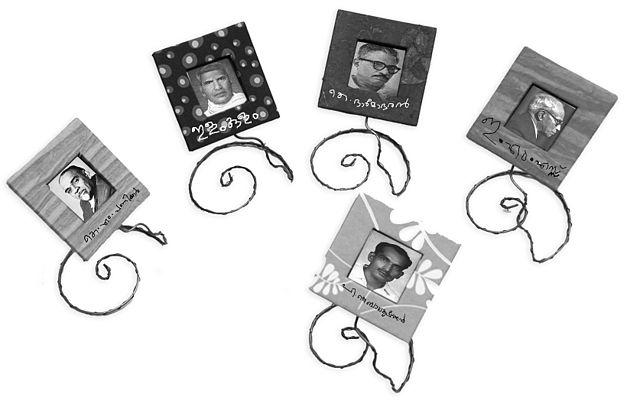
\includegraphics[width=8cm,height=6cm]{Kulasthree_Chapter01_pic07.jpg}
\end{center}
\end{figure}

\paragraph{}	കേരളത്തിൽ ഇന്നു ലഭ്യമായ ചരിത്രപഠനങ്ങളിൽ സ്ത്രീകളുടെ സാന്നിദ്ധ്യം എത്രത്തോളമുണ്ട്? പുരാതന-മദ്ധ്യകാലങ്ങളിലെ സ്ത്രീകളെപ്പറ്റി പല പരാമർശങ്ങളും ലഭ്യമായ ചരിത്രസാമഗ്രികളിലുണ്ടെങ്കിലും ഈ പ്രദേശത്തെ പുരാതന-മദ്ധ്യകാല സാമൂഹ്യസാഹചര്യങ്ങളെ സ്ത്രീചരിത്രരചനയുടെ കണ്ണുകളിലൂടെ വിലയിരുത്തുന്ന വിപുലമായ പഠനങ്ങൾ ഇനിയുമുണ്ടായിട്ടില്ല എന്നതാണ് സത്യം. "കേരളത്തിലെ സ്ത്രീകളുടെ പഴയനില വളരെ മെച്ചമായിരുന്നു; അതിന് തെളിവാണ് വടക്കൻപാട്ടുകളിലെ ഉണ്ണിയാർച്ചയുടെ കഥ" എന്നൊക്കെ ചില പ്രസംഗങ്ങളിലും മറ്റും നാം കേൾക്കാറുണ്ട്. ഈ പ്രസ്താവത്തിന് തീരെ ബലംപോരെന്നു പറയാതെ വയ്യ. ഒരു ഉണ്ണിയാർച്ചയെയല്ലേ നാം കണ്ടുള്ളൂ? അതിൽനിന്നും ഇവിടത്തെ സ്ത്രീകളെല്ലാവരും പയറ്റിത്തെളിഞ്ഞവരായിരുന്നുവെന്ന് കരുതുന്നത് ശരിയോ? അന്നത്തെ സമൂഹത്തിൽ പല തട്ടുകളിൽ ജീവിച്ച സ്ത്രീകളെപ്പറ്റിയുള്ള വിവരങ്ങൾ ശേഖരിച്ചുകൊണ്ടുള്ള ചിട്ടയായ ചരിത്രരചന ഇനിയും നടക്കാനിരിക്കുന്നതേയുള്ളുവെന്നതാണ് വസ്തുത.

\paragraph{}	പക്ഷേ, മറ്റൊരുവിധത്തിൽ സ്ത്രീകൾ പലപ്പോഴും "നിഷ്പക്ഷകേരളചരിത്ര'ത്തിൽ പ്രത്യക്ഷപ്പെടുന്നുണ്ടെന്നതാണ് കൗതുകകരമായ കാര്യം. ഒരു സമൂഹത്തിന്റെ അവസ്ഥയെ വിലയിരുത്താനുള്ള എളുപ്പവഴി, അവിടുത്തെ സ്ത്രീകളുടെ നിലയെക്കുറിച്ച് അന്വേഷിക്കലാണെന്ന വിശ്വാസം വളരെ മുമ്പേ നമ്മുടെയിടയിൽ പ്രചാരത്തിലുള്ള ഒന്നാണ്. ഒറ്റനോട്ടത്തിൽ ഇതു സ്ത്രീകൾക്ക് ലഭിച്ച അഭിനന്ദനമാണെന്നു തോന്നിയേക്കാം. പക്ഷേ, കൂടുതലാലോചിച്ചാൽ ഈ അഭിനന്ദനം സമൂഹത്തിന്റെ നന്മ, സദാചാരം, പുരോഗതി മുതലായവയ്ക്കുള്ള ഉത്തരവാദിത്വത്തിന്റെ കൂടുതൽഭാഗം സ്ത്രീകളിൽ നിക്ഷിപ്തമാക്കുന്നുവെന്ന് കാണാം. 'നിഷ്പക്ഷചരിത്ര'ത്തിൽ സ്ത്രീകൾ ഇത്തരമൊരു അളവുകോലായിമാത്രം പ്രത്യക്ഷപ്പെടുന്നു. സ്ത്രീകളുടെ വിദ്യാഭ്യാസം, ആരോഗ്യം തുടങ്ങിയ കാര്യങ്ങളെക്കുറിച്ചുള്ള കണക്കുകൾ അവതരിപ്പിച്ചുകൊണ്ട് ആ സമൂഹത്തിന്റെ നിലയെക്കുറിച്ച് "നിഷ്പക്ഷചരിത്ര'രചയിതാക്കൾ നിഗമനങ്ങളിലെത്തും. അക്കാലങ്ങളിലെ സ്ത്രീകളുടെ ചരിത്രാനുഭവങ്ങളെക്കുറിച്ച് ഇതിലധികമൊന്നും പറയാനില്ലെന്ന മട്ടിൽ! സമൂഹത്തിനു മൊത്തത്തിലുണ്ടായ നേട്ടങ്ങൾക്കു പുറമെ സ്ത്രീകൾക്ക് ഇത്തരം മാറ്റങ്ങൾ എന്തു ഗുണംചെയ്തു? ഇവയിലൂടെ സ്ത്രീകൾക്ക് സമൂഹം കൽപ്പിക്കുന്ന വില, അവരുടെ സാമൂഹ്യനില, സ്വാതന്ത്ര്യങ്ങൾ മുതലായവയിൽ ക്രിയാത്മകമായ മാറ്റങ്ങൾ ഉണ്ടായോ? ഈ ചോദ്യങ്ങൾക്ക് കുറഞ്ഞ പ്രാധാന്യംമാത്രമേ നിഷ്പക്ഷചരിത്രകാരന്മാർ കൽപ്പിക്കുന്നുള്ളൂ. ചിലപ്പോൾ തികഞ്ഞ പുരുഷമേധാവിത്വപരമായ മൂല്യങ്ങളാണ് ഈ വിലയിരുത്തലിൽ പ്രവർത്തിക്കുക. മരുമക്കത്തായത്തോട് പലരും പുലർത്തുന്ന മനോഭാവംതന്നെയെടുക്കുക. സ്ത്രീകൾക്ക് വിവാഹത്തിൽ കൂടുതൽ അധികാരങ്ങൾ നൽകുകയും ലൈംഗികകാര്യങ്ങളിൽ അവരുടെ ഇഷ്ടത്തിനും അഭിപ്രായത്തിനും താരതമ്യേന കൂടുതൽ വില കൽപ്പിക്കുകയും കുടുംബസ്വത്തിന്റെ അവകാശം പെൺവഴിക്ക് നീങ്ങുന്ന കുടുംബങ്ങൾ പുലരുകയും ചെയ്തിരുന്ന മരുമക്കത്തായവ്യവസ്ഥ കേരളചരിത്രകാരന്മാരിൽ ഒരുകാലത്ത് ഇത്രയേറെ അസ്വസ്ഥത സൃഷ്ടിച്ചതെന്തുകൊണ്ടെന്ന കാര്യം പഠിക്കേണ്ടതുതന്നെ! പക്ഷേ, മരുമക്കത്തായത്തെ പുനർമൂല്യംചെയ്യാൻ തയ്യാറായവർപോലും സ്ത്രീകളുടെ ചരിത്രത്തെ സാമൂഹ്യസ്ഥാപനങ്ങളുടെ ചരിത്രത്തിലേക്കു ചുരുക്കുന്നതിലെ അപകടം തിരിച്ചറിഞ്ഞില്ല.

\paragraph{}	സാമൂഹ്യസ്ഥാപനങ്ങൾക്ക് കേവലം കീഴ്പ്പെട്ടതാണ് സ്ത്രീകളുടെ ജീവിതമെന്ന ധാരണയെ പുതിയ സ്ത്രീചരിത്രം എതിർക്കുന്നു. സ്ഥാപനങ്ങൾക്കുള്ളിൽ ജീവിക്കുമ്പോഴും സ്ത്രീകൾ നിഷ്ക്രിയരായിരുന്നില്ലെന്ന് സ്ത്രീപക്ഷഗവേഷണം തെളിയിക്കുന്നു. കുടുംബത്തിന്റെയും സമുദായത്തിന്റെയും നിയമങ്ങൾക്കു കീഴ്പ്പെട്ടുകഴിയുന്ന സ്ത്രീകൾ ആ നിയമങ്ങളെ നേരിട്ടോ അല്ലാതെയോ മറികടക്കാൻ സജീവശ്രമങ്ങളിൽ ഏർപ്പെട്ടിരുന്നു; ഇന്നും ഏർപ്പെടുന്നു. ഈ സ്ഥാപനങ്ങൾ സ്ത്രീകൾക്കു കൽപ്പിക്കുന്ന പരിധികളെ സ്ഥാപനത്തിനുള്ളിൽനിന്നുകൊണ്ട് വിസ്തൃതമാക്കാൻ അവർ എന്നും ശ്രമിച്ചിട്ടുണ്ട്. ഈ സമ്പന്നമായ ചരിത്രാനുഭവത്തിന് തുച്ഛമായ വിലമാത്രം കൽപ്പിക്കുന്ന 'നിഷ്പക്ഷ'ചരിത്രത്തെ സ്ത്രീപക്ഷചരിത്രത്തിന്റെ വക്താക്കൾ തള്ളിക്കളഞ്ഞതു വെറുതെയല്ല.

\paragraph{} മാർക്സിസ്റ്റ് ചരിത്രരചനാരീതി മേലാള ചരിത്രത്തെ തുറന്നെതിർക്കുന്നുണ്ട്. എങ്കിലും കേരളത്തിൽ ഈ പാത പിന്തുടർന്നവരുടെ പഠനങ്ങളിലും സ്ത്രീകൾ ഏറെക്കുറെ അദൃശ്യർതന്നെ. ഭൂതകാലത്തിലുടനീളം ഉള്ളവരും ഇല്ലാത്തവരും തമ്മിൽ സംഘർഷത്തിലായിരുന്നുവെന്നും അത് പഠിക്കുന്നതിലൂടെ ഭാവികാലം രൂപപ്പെടുന്നതിനെപ്പറ്റി പല ഉൾക്കാഴ്ചകളും നമുക്ക് കിട്ടുമെന്നും മാർക്സിസ്റ്റ് ചരിത്രകാരന്മാർ അവകാശപ്പെടുന്നു. അതുപോലെ സമൂഹത്തിൽ സമ്പത്തുണ്ടാക്കുന്ന രീതികളിലുണ്ടാകുന്ന മാറ്റങ്ങൾക്കനുസരിച്ച് ഉള്ളവരുടെയും ഇല്ലാത്തവരുടെയും ജീവിതങ്ങളിൽ മാറ്റമുണ്ടാകുന്നുവെന്നും അവർ ചൂണ്ടിക്കാണിക്കുന്നു. അപ്പോൾ ഈ സംഘർഷങ്ങളിൽ ജീവിതഗതികൾക്കുണ്ടാകുന്ന മാറ്റങ്ങളിൽ സ്ത്രീകളുടെ നിലയെന്താണ്? സ്ത്രീകളുടെ നില മേൽപ്പറഞ്ഞ വർഗ്ഗസംഘർഷത്തിന് കീഴ്വഴങ്ങിനിൽക്കുന്നുവെന്നാണ് മാർക്സിസ്റ്റ് ചരിത്രകാരന്മാർ പൊതുവേ കരുതുന്നത്; വർഗ്ഗസംഘർഷത്തിന്റെ ഗതിയനുസരിച്ച് അതു മാറുമെന്നും. ഈ ആശയത്തെ സ്ത്രീ ചരിത്രരചനയിലേർപ്പെടുന്നവർ ചോദ്യംചെയ്യുന്നു. പുരുഷന് സ്ത്രീക്കുമേൽ കൈവന്ന അധികാരം വർഗ്ഗസമരങ്ങളുടെ മുറയ്ക്ക് മാറിക്കൊള്ളണമില്ലെന്ന് അവർ വാദിക്കുന്നു. മാർക്സിസ്റ്റ് ചരിത്രത്തിന്റെ ഉൾക്കാഴ്ചകളെ മൊത്തത്തിൽ അംഗീകരിക്കുന്നുണ്ടെങ്കിലും സാമ്പത്തികമാറ്റങ്ങൾക്ക് അതിനുള്ളിൽ കൽപ്പിക്കപ്പെടുന്ന അമിതപ്രാധാന്യം ഗുണകരമല്ലെന്ന് സ്ത്രീപക്ഷചരിത്രം ചൂണ്ടിക്കാണിക്കുന്നു. സാമൂഹ്യസ്ഥാപനങ്ങളും ആശയവ്യവസ്ഥകളും പലപ്പോഴും സാമ്പത്തികമാറ്റങ്ങളെ അതിജീവിക്കുകയും സമ്പദ്‌വ്യവസ്ഥയിലെ ചലനങ്ങൾക്കനുസരിച്ച് പുതിയ ധർമ്മങ്ങൾ കൈക്കൊള്ളുകയും ചെയ്യുന്നത് ശ്രദ്ധേയമാണെന്ന് അവർ ഓർമ്മിപ്പിക്കുന്നു. ഇന്നു നാം പലയിടത്തും കാണുന്ന 'തറവാടിത്തഘോഷണം' നല്ലൊരു ഉദാഹരണമാണ്. മേൽജാതിക്കാരുടെ ആഭിജാത്യചിഹ്നങ്ങളായ പലതും - തറവാട്, കോടിവസ്ത്രം, പലതരത്തിലുള്ള മര-ലോഹസാമാനങ്ങൾ മുതലായവ - അവയുടെ പഴയ ധർമ്മം കൈവെടിഞ്ഞ് മുതലാളിത്ത വ്യവസ്ഥയ്ക്കുള്ളിൽ പുതിയ മൂല്യങ്ങൾ സ്വീകരിച്ചിരിക്കുന്നു. ഓണക്കാലത്തും മറ്റും ടെലിവിഷനിലൂടെ നാം കാണുന്ന 'പാരമ്പര്യം' വാസ്തവത്തിൽ പഴമയല്ല; നവവരേണ്യവർഗ്ഗത്തിന്റെ പുതിയ (മുതലാളിത്ത) മൂല്യങ്ങൾക്കനുസൃതമായ രീതിയിൽ വാർത്തെടുക്കപ്പെട്ടവയാണ്. അതു പോലെ, സമൂഹത്തിൽ വിഭവങ്ങളുണ്ടാക്കുന്ന രീതികൾ, സാമ്പത്തിക ഇടപാടുകൾക്കുണ്ടാകുന്ന മാറ്റം ഇതെല്ലാം സ്ത്രീകളുടെ ജീവിതത്തെ കാര്യമായി ബാധിക്കുമെന്ന് അംഗീകരിച്ചുകൊണ്ടുതന്നെ സ്ത്രീചരിത്രരചനയിലേർപ്പെടുന്നവർ പറയുന്നു: 'പക്ഷേ, ഇത്തരം മാറ്റങ്ങൾ എല്ലാവരെയും ഒരുപോലെയല്ല ബാധിക്കുന്നത്. മേലാളരിൽത്തന്നെ സ്ത്രീക്കും പുരുഷനും വ്യത്യസ്ത അനുഭവങ്ങളായിരിക്കും ഉണ്ടാക്കുക. കീഴാളസ്ത്രീ-പുരുഷന്മാരുടെ അനുഭവങ്ങൾ തമ്മിലും വ്യത്യാസങ്ങളുണ്ടാകാം. കൂടാതെ മേലാളസ്ത്രീകളും കീഴാളസ്ത്രീകളും ഈ സാഹചര്യങ്ങളെ അഭിമുഖീകരിച്ചത് തീർത്തും വ്യത്യസ്ത രീതികളിലായിരിക്കാം. ഈ വ്യത്യാസങ്ങളുടെ പ്രാധാന്യം കുറച്ചു കണ്ടുകൂടാ, 'നിഷ്പക്ഷ'ചരിത്രത്തിന്റെ അല്ലെങ്കിൽ ശാസ്ത്രീയചരിത്രത്തിന്റെ പേരുപറഞ്ഞ് അവയെ കണ്ടില്ലെന്നു നടിച്ചുകൂടാ.'

\begin{figure}[h]
\begin{center}
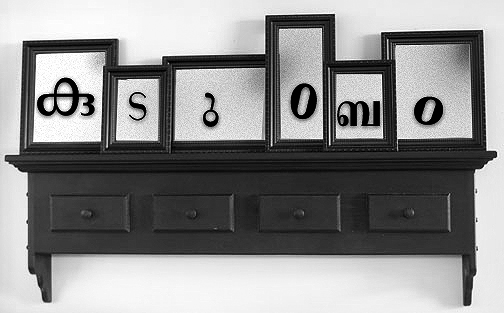
\includegraphics[width=\textwidth,height=5cm]{Kulasthree_Chapter01_pic08.jpg}
\end{center}
\end{figure}

\paragraph{}	കേരളചരിത്രത്തിന്റെ പ്രാചീനഘട്ടത്തെയും മദ്ധ്യകാലത്തെയും സ്ത്രീപക്ഷവീക്ഷണത്തിൽ വിലയിരുത്തുന്ന പഠനങ്ങൾ ഇന്നു കുറവാണ്. പക്ഷേ ആധുനികകാലത്തെക്കുറിച്ച് കുറേക്കൂടി പഠനങ്ങളുണ്ട്. ഇവിടെ പുതിയ സ്ത്രീചരിത്രവും ആൺ-പെൺഭേദത്തിന്റെ ചരിത്രവും ചർച്ചചെയ്യപ്പെടുന്നുണ്ട്. അതുകൊണ്ടുതന്നെ പത്തൊമ്പതാംനൂറ്റാണ്ടിന്റെ ഏതാണ്ട് പകുതിമുതൽ ഇരുപതാം നൂറ്റാണ്ടുവരെയുണ്ടായ മാറ്റങ്ങളാണ് ഈ പുസ്തകത്തിൽ അധികവും ചർച്ചചെയ്യപ്പെടുന്നത്. മലയാളിസ്ത്രീയുടെ "വിമോചനയുഗ'മായി ഈ കാലത്തെ പറയാറുണ്ട്. തെക്കൻകേരളത്തിലെ ചാന്നാർ സ്ത്രീകൾക്ക് മേൽമുണ്ടു ധരിക്കാനുള്ള അവകാശത്തെ ചുറ്റിപ്പറ്റി പത്തൊമ്പതാം നൂറ്റാണ്ടിൽ നടന്ന കലാപങ്ങളെ ആദ്യത്തെ സ്ത്രീവിമോചനസമരമായി കാണുന്നരീതി പതിവാണ്. ഇരുപതാംനൂറ്റാണ്ടിലെത്തിയപ്പോൾ സാമുദായികപ്രസ്ഥാനങ്ങളുടെ ശ്രമഫലമായി സ്ത്രീകളുടെ നില കൂടുതൽ മെച്ചപ്പെട്ടുവെന്നാണ് സാധാരണ നാം കേൾക്കാറുള്ളത്. പകുതിസത്യം മുഴുത്ത കള്ളത്തെക്കാൾ ദോഷംചെയ്യുമെന്ന് പ്രസിദ്ധമാണല്ലോ. ഈ പകുതിസത്യങ്ങളെ വിമർശനപരമായി പുനർവിചാരണചെയ്തും പുതിയ തെളിവുകൾ കണ്ടെത്തിയും പഴയ തെളിവുകളെ പുതിയ കാഴ്ചപ്പാടിൽ വിലയിരുത്തിയുമാണ് സ്ത്രീചരിത്രം ഇവിടെ പുതിയ ഉൾക്കാഴ്ചകളുണ്ടാക്കുന്നത്. 1950കൾക്കുമുമ്പ് തിരുവിതാംകൂർ, കൊച്ചി, മലബാർ എന്നിങ്ങനെ വേർതിരിഞ്ഞുകിടന്ന പ്രദേശങ്ങളെ ഒന്നിച്ചുചേർത്താണ് മലയാളഭാഷ സംസാരിക്കുന്നവരുടെ സംസ്ഥാനമായ കേരളം നിലവിൽവന്നത്. ഇതിൽ തിരുവിതാംകൂറും കൊച്ചിയും ബ്രിട്ടിഷ്സാമ്രാജ്യത്തിന്റെ മേൽക്കോയ്മ അംഗീകരിച്ച നാട്ടുരാജ്യങ്ങളായിരുന്നു. മലബാർഭാഗം ബ്രിട്ടിഷുകാർ നേരിട്ടു ഭരണംനടത്തിവന്ന മദ്രാസ് പ്രവിശ്യയുടെ ഭാഗമായിരുന്നു. ഈ പുസ്തകം തിരുവിതാംകൂറിൽ നടന്ന കാര്യങ്ങൾക്ക് കൂടുതൽ പ്രാധാന്യം നൽകുന്നു. ബ്രിട്ടിഷ് മേൽക്കോയ്മയ്ക്കു മുന്നിൽ പിടിച്ചുനിൽക്കാനൊരു തന്ത്രമെന്ന നിലയിൽ സ്ത്രീകളുടെ വിദ്യാഭ്യാസം, ആരോഗ്യം മുതലായ വിഷയങ്ങളിൽ തിരുവിതാംകൂറിലെയും കൊച്ചിയിലെയും സർക്കാരുകൾ സവിശേഷതാത്പര്യം പ്രകടിപ്പിച്ചിരുന്നു. സ്ത്രീകളുടെ അവകാശങ്ങൾ, ലിംഗബന്ധങ്ങൾ മുതലായ വിഷയങ്ങൾ ഏറ്റവും വ്യാപകമായി ചർച്ചചെയ്യപ്പെട്ടതും ഇവിടെത്തന്നെ.

\paragraph{}	മലബാറിൽ ഇത്തരം ചർച്ചകൾ തീരെ നടന്നിരുന്നില്ലെന്നല്ല. മരുമക്കത്തായത്തിന്റെ ഗുണദോഷങ്ങളെപ്പറ്റി വളരെ സജീവമായ ചർച്ച മലബാറിൽ പത്തൊമ്പതാം നൂറ്റാണ്ടിന്റെ അവസാനകാലത്തും ഇരുപതാംനൂറ്റാണ്ടിലുമായി നടന്നിട്ടുണ്ട്. ഇന്ത്യയിലെ ആദ്യത്തെ സ്ത്രീസംഘടനകളിലൊന്നായിരുന്ന അഖിലേന്ത്യാ വനിതാകോൺഫറൻസിന്റെ ഒരു ഘടകം മലബാറിൽ നന്നായി പ്രവർത്തിച്ചിരുന്നു. സ്വാതന്ത്ര്യസമരത്തിലും കമ്മ്യൂണിസ്റ്റുപ്രസ്ഥാനത്തിലും മലബാറിലെ സ്ത്രീകൾ സജീവ പങ്കാളികളായിരുന്നു. എന്നാൽ തിരുവിതാംകൂർ-കൊച്ചി രാജ്യങ്ങളിൽ പൊതുകാര്യങ്ങളെക്കുറിച്ചു ചർച്ച നടന്നിരുന്ന വേദികൾ - പൊതുമണ്ഡലങ്ങൾ - കൂടുതൽ വികസിതങ്ങളായിരുന്നതുകൊണ്ടും അവ നാട്ടുരാജ്യങ്ങളായിരുന്നതിനാൽ ദേശീയപ്രസ്ഥാനത്തിന്റെ സമ്മർദ്ദം താരതമ്യേന കുറവായിരുന്നതുകൊണ്ടും അവിടങ്ങളിൽ സ്ത്രീകളുടെ അവകാശങ്ങളെക്കുറിച്ചുള്ള ചർച്ച കൂടുതൽ ആഴത്തിൽ നടന്നുവെന്നു പറയാം. (സ്വാതന്ത്ര്യസമരം ശക്തമായ ഭാഗങ്ങളിൽ ദേശീയസ്വാതന്ത്ര്യം നേടുന്നതിന്റെ പ്രശ്നങ്ങൾക്കും വഴികൾക്കുമാണ് പലപ്പോഴും മുൻതൂക്കം ലഭിച്ചത്)

\paragraph{}	പത്രങ്ങൾ, ചർച്ചാവേദികൾ, സമുദായപരിഷ്കരണസംഘങ്ങൾ, സാമൂഹ്യസേവനസ്ഥാപനങ്ങൾ, വായനശാലകൾ, വിദ്യാലയങ്ങളിലും മറ്റും ആരംഭിച്ച സാഹിത്യസമാജങ്ങൾ, സാഹിത്യവേദികൾ, വനിതാസമാജങ്ങൾ, യുവജനസംഘടനകൾ മുതലായ പല കൂട്ടായ്മകളും ചേർന്നാണ് 'പൊതുമണ്ഡലം' രൂപീകരിക്കപ്പെടുന്നത്. ജനങ്ങളെ 'പൊതു'വായി ബാധിക്കുന്ന കാര്യങ്ങൾ ചർച്ച ചെയ്യാനുള്ള വേദിയാണത്. ജാതി-സമുദായങ്ങളുടെ സീമകളെ അതിലംഘിക്കുന്ന തരത്തിലുള്ള കാര്യങ്ങളും ചർച്ചകളുമാണ് 'പൊതുമണ്ഡല'ത്തിൽ വരുന്നതെന്ന് ഒറ്റനോട്ടത്തിൽ തോന്നിയേക്കാം. എന്നാൽ സ്ത്രീകൾക്കും പുരുഷന്മാർക്കും മേൽജാതിക്കാർക്കും കീഴ്ജാതിക്കാർക്കും ഒരുപോലെ കയറിച്ചെല്ലാവുന്ന ഇടമായിരുന്നില്ല അത്. സ്ത്രീകൾ 'സ്ത്രീസമാജ'ങ്ങളിലും പുരുഷന്മാർ 'പൗരസമാജ'ങ്ങളിലും ഒത്തുചേരുന്നതാണ് ഉത്തമം എന്ന ബോധം മലയാളിപൊതുമണ്ഡലത്തിൽ അന്നും ഇന്നും സജീവമാണ്.

\paragraph{}	ഇന്നത്തെ കേരളത്തിൽ നിരവധി വെല്ലുവിളികളെ നേരിടുന്ന സ്ത്രീകൾക്ക് ചോദിക്കാൻ ഒരുപാടു ചോദ്യങ്ങളുണ്ട്. വിദ്യാഭ്യാസം, പ്രസവം, ആരോഗ്യം, കുടുംബാസൂത്രണം എന്നീ മേഖലകളിൽ ഇരുപതാംനൂറ്റാണ്ടിലെ മലയാളിസ്ത്രീകൾക്കുണ്ടായ നേട്ടങ്ങളെപ്പറ്റി പലയിടത്തും ഇന്ന് പറഞ്ഞുകേൾക്കാറുണ്ട്; വായിച്ചുകാണാറുണ്ട്. സ്ത്രീസാക്ഷരതയിലും വിദ്യാഭ്യാസത്തിലും ഒരു കുതിച്ചുചാട്ടംതന്നെയാണ് ഈ നൂറ്റാണ്ടിലുണ്ടായത്. ഇതുകൂടാതെ സ്ത്രീകൾ സർക്കാർജോലികളിലും മറ്റും പ്രവേശിച്ചു, ദേശീയപ്രസ്ഥാനത്തിലും ഇടതുപക്ഷപ്രസ്ഥാനത്തിലും പങ്കെടുത്തു, ഇവിടത്തെ ഏറ്റവും വലിയ തൊഴിലാളിസംഘടനകളിൽ ചേർന്ന് തൊഴിൽസമരങ്ങളുടെ മുൻനിരയിൽ പ്രത്യക്ഷപ്പെട്ടു. ഈ നേട്ടങ്ങളെല്ലാമുണ്ടായിട്ടും നമ്മുടെ നില ഇത്ര മോശമായിരിക്കുന്നതെന്തുകൊണ്ടെന്ന ചോദ്യം ഓരോ മലയാളിസ്ത്രീയുടെയുമുള്ളിൽ നിശബ്ദമുയരുന്ന ഇക്കാലത്ത് ഈ പുസ്തകം ഏറ്റവും പ്രസക്തമാണെന്ന് കരുതുന്നു.

\paragraph{} മറ്റൊരു പ്രചോദനംകൂടിയുണ്ട് ഈ പുസ്തകത്തിനു പിന്നിൽ. കേരളത്തിലെ മറ്റേതു രാഷ്ട്രീയപ്രസ്ഥാനത്തിനും - ഇടതുപക്ഷപ്രസ്ഥാനമാകട്ടെ, കോൺഗ്രസ്സാകട്ടെ, കീഴ്ജാതിക്കാരുടെ അവകാശങ്ങൾ നേടിയെടുക്കാനുളള പ്രസ്ഥാനങ്ങളാകട്ടെ - ഒരു ചരിത്രപാരമ്പര്യം അവകാശപ്പെടാനുണ്ട്. എന്നാൽ സ്ത്രീകളുടെ അവകാശങ്ങൾക്കുവേണ്ടി വാദിക്കുന്ന പ്രസ്ഥാനത്തിന്റെ ചരിത്രത്തെക്കുറിച്ച് അധികമാരും പറഞ്ഞുകേൾക്കാറില്ല. വാസ്തവത്തിൽ വലിയൊരു അന്യായമാണിത്. കേരളത്തിൽ സ്ത്രീപക്ഷത്തുനിന്നുള്ള ശബ്ദങ്ങൾ കേട്ടുതുടങ്ങിയത് 1980കളിലാണെന്ന ധാരണ ശരിയല്ല. അതിനെത്രയോ മുമ്പുതന്നെ ഇവിടെ സ്ത്രീകളുടെ അവകാശങ്ങൾക്കുവേണ്ടി അതിശക്തമായ ഭാഷയിൽ വാദിച്ച സ്ത്രീബുദ്ധിജീവികളുടെ ഒരു തലമുറതന്നെയുണ്ടായിരുന്നു. 1920കൾ മുതൽ 1940കൾ വരെ കേരളത്തിന്റെ പൊതുരംഗത്ത് ഇവർ സജീവസാന്നിദ്ധ്യമായിരുന്നു. ഈ തലമുറ അന്യംനിന്നുപോയതെങ്ങനെ, ഇവരുടെ സ്മരണപോലും നമുക്കില്ലാതെപോയതെന്തുകൊണ്ട് തുടങ്ങിയ ചോദ്യങ്ങൾ ചോദിക്കേണ്ടതാണ്. കാരണം, നമ്മൾ 'പഴയകാലത്തെ പ്രമുഖസ്ത്രീകൾ' എന്നോർക്കുന്നത് ദേശീയപ്രസ്ഥാനത്തിലോ ഇടതുപക്ഷപ്രസ്ഥാനത്തിലോ പ്രവർത്തിച്ച സ്ത്രീകളെക്കുറിച്ചാണ്. എന്നാൽ സ്ത്രീകളെ ഒരു പ്രത്യേകവിഭാഗമായിക്കരുതി അവരുടെ അവകാശങ്ങൾക്ക് സവിശേഷപരിഗണന നൽകണമെന്നു വാദിച്ച സ്ത്രീകൾ ഈ നാട്ടിലുണ്ടായിരുന്നുവെന്ന കാര്യം എത്രപേർക്കറിയാം? അവരിൽ ചിലരെക്കുറിച്ച് നാം ചിലപ്പോൾ കേട്ടിട്ടുണ്ടാവും. ഉദാഹരണത്തിന് അന്നാ ചാണ്ടി. ഇന്ത്യയിൽ ആദ്യമായി മുൻസിഫ് പദവിയിലെത്തിയ സ്ത്രീ എന്നാണ് നമുക്ക് ഇവരെപ്പറ്റിയുളള അറിവ്. എന്നാൽ കേരളീയസ്ത്രീകളുടെ അവകാശങ്ങൾക്കുവേണ്ടി പോരാടിയ വനിതകളിൽ ഇവർക്കുണ്ടായിരുന്ന പ്രമുഖസ്ഥാനത്തെപ്പറ്റി എത്രപേർ കേട്ടിട്ടുണ്ട്?
അന്നത്തെ കൊമ്പുകെട്ടിയ പുരുഷബുദ്ധിജീവികളുടെ പുരുഷാധികാരപരമായ നിലപാടുകളെ വിമർശിച്ചുകൊണ്ടും തുറന്നെതിർത്തുകൊണ്ടും ഇവരെഴുതിയ ലേഖനങ്ങളിൽ പലതും ഇന്നത്തെക്കാലത്തും പ്രസക്തങ്ങളാണ്. സ്ത്രീപക്ഷത്തുനിന്നു വാദിച്ച സ്ത്രീകളുടെ ആ തലമുറ കുറ്റമറ്റതാണെന്നോ അവരുമായി നാം പൂർണ്ണമായും യോജിക്കുമെന്നോ അല്ല. തീർച്ചയായും അവർക്ക് പോരായ്മകളുണ്ടായിരുന്നു. എങ്കിലും അവരിൽനിന്ന് ചിലതൊക്കെ പഠിക്കാനുണ്ട്. യുക്തിയും നർമ്മബോധവും സമകാലികപ്രശ്നങ്ങളെപ്പറ്റിയുളള അറിവും വേണ്ടവിധം കൂട്ടിച്ചേർത്ത് അവർ നിർമ്മിച്ച ശക്തമായ വാദശൈലി ഒരുദാഹരണംമാത്രമാണ്. അധികാരസ്ഥാനത്തിരിക്കുന്ന വ്യക്തികളെയോ അധികാരസ്ഥാപനങ്ങളെയോ തീരെ ഭയക്കാതെ, പറയാനുളള കാര്യം ശക്തവും വ്യക്തവുമായ ഭാഷയിൽ പറയാനുള്ള ആ തന്റേടം തീർച്ചയായും ഇന്നു നമുക്കില്ല. ആ തലമുറയെ ഇന്നത്തെ സ്ത്രീപുരുഷന്മാർക്ക് പരിചയപ്പെടുത്തുകയെന്ന ലക്ഷ്യംകൂടി ഈ പുസ്തകത്തിനുണ്ട്. ആ തലമുറയ്ക്ക് ഇനിയുള്ള കാലത്ത് പുതിയ അവകാശികൾ ഒരുപാടുണ്ടാകുമെന്ന പ്രത്യാശയാണ് ഈ പുസ്തകത്തെ നയിക്കുന്നത്; അവർ ഈ വിമർശനപാരമ്പര്യത്തെ കാലാനുസൃതമായി നവീകരിക്കുമെന്നും. 

\begin{figure}[h]
\begin{center}
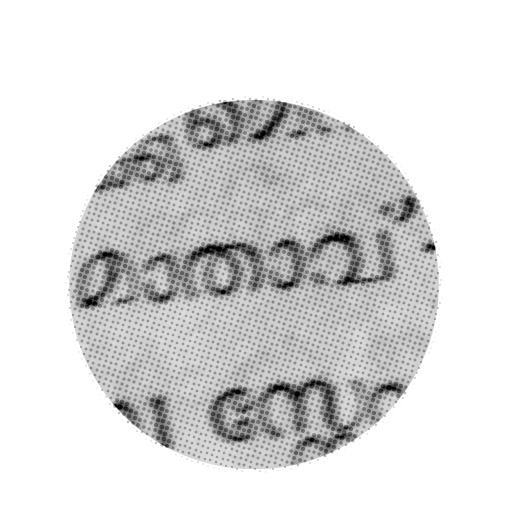
\includegraphics[width=3cm,height=5cm]{Kulasthree_Chapter01_pic09.jpg}
\end{center}
\end{figure}